\documentclass{package/fancy-book}
\setlength{\parindent}{2em}
\usepackage[UTF8]{ctex}

%%%%%%%%%% Default Package %%%%%%%%%%%%%
\usepackage{package/color-env}
\usepackage{package/quiver}
\usepackage{background}
\usepackage[object=vectorian]{pgfornament} %% used in title.tex
\usepackage{calligra} %%% (optional) to make the Title text beautiful 
\usepackage{lipsum}  %% for dummy text 
\usepackage{amssymb,amsmath,amsfonts}  %%% for maths
\usepackage{datetime}
%%%%%% Optional Packages %%%%%%%
\usepackage{lettrine} %% for nice looking 
\usepackage{GoudyIn} %% first Letter of the paragraph
\renewcommand{\LettrineFontHook}{\color{black}\GoudyInfamily{}}
\LettrineTextFont{\itshape}
\setcounter{DefaultLines}{3}%
%%%%%%%%%%%%%%%%%%%%%%%%%%%%%%%%%%%%%
\usepackage{datetime2}
\usepackage{fourier-orns}
\newcommand{\ornamento}{\vspace{2em}\noindent \textcolor{darkgray}{\hrulefill~ \raisebox{-2.5pt}[10pt][10pt]{\leafright \decofourleft 
\decothreeleft  \aldineright \decotwo \floweroneleft \decoone   \floweroneright 
\decotwo \aldineleft\decothreeright \decofourright \leafleft} ~  \hrulefill \\ \vspace{2em}}}

%定义命令
\newcommand{\N}{\mathbb{N}}
\newcommand{\Z}{\mathbb{Z}}
\newcommand{\Q}{\mathbb{Q}}
\newcommand{\R}{\mathbb{R}}
\newcommand{\C}{\mathbb{C}}
\newcommand{\HH}{\mathbb{H}}
\newcommand{\RP}{\mathbb{RP}}

%%%% Bibliography %%%%%%%%%
% Required packages are included in notes class
% Can be tweaked in the notes.cls file itself
\addbibresource{resource/references.bib}
\newcommand{\id}{\mathrm{id}}
\newcommand{\Hom}{\mathrm{Hom}}
\begin{document}
\begin{titlepage}

%%%%%%%%%%%%%%%%%%%%%%%%%%%%%%%%%%%% Inspired From  %%%%%%%%%%%%%%%%%%%%%%%%%%%%%%%%%%%%%%%%%%%%%%%%% 
%%%%  https://www.reddit.com/r/LaTeX/comments/j9d739/hello_world_in_latex_is_a_lot_cooler/   %%%%%
%%%%%%%%%%%%%%%% If this doesn't look nice then you may remove it %%%%%%%%%%%%%%%%%%%%%%%%%%

\backgroundsetup{
scale=1,
opacity=1,
angle=0,
color=black,
contents={
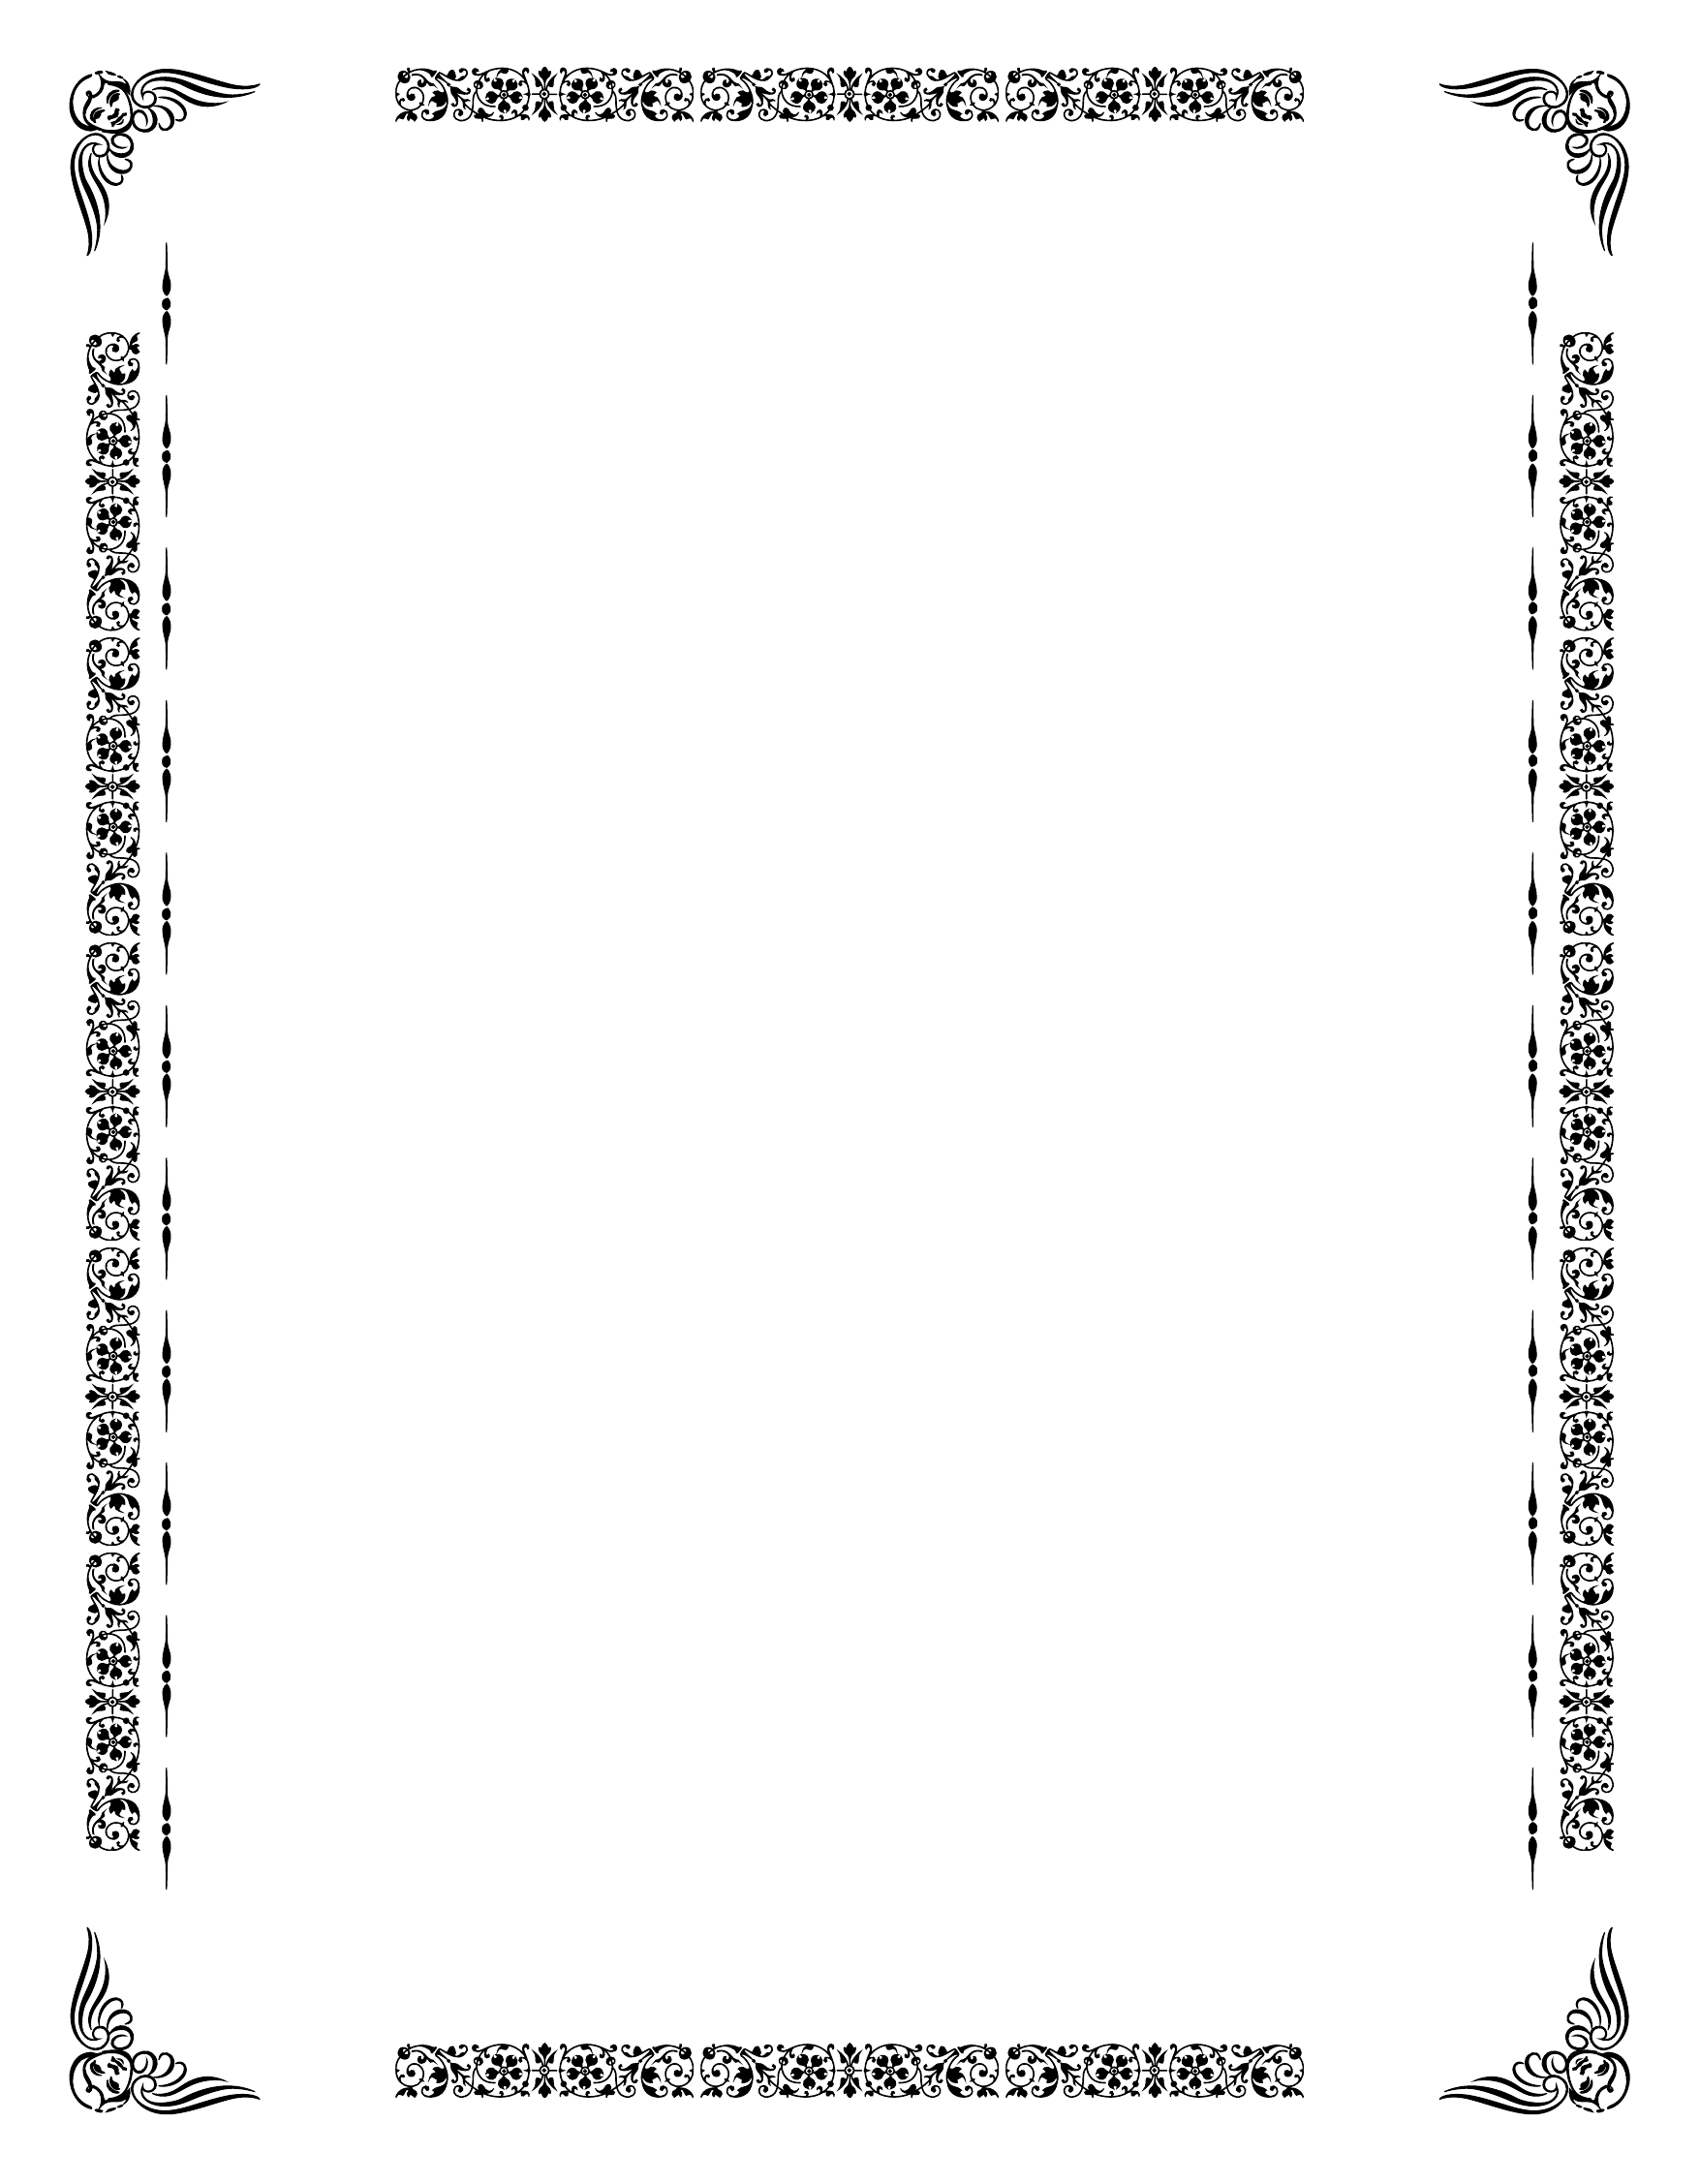
\begin{tikzpicture}[color=black, every node/.style={inner sep= 15pt}]
\node (NW) [anchor=north west] at (current page.north west){\pgfornament[width=2.5cm] {131}};
\node (NE) [anchor=north east] at (current page.north east){\pgfornament[width=2.5cm, symmetry=v]{131}};
\node (SW) [anchor=south west] at (current page.south west){\pgfornament[width=2.5cm, symmetry=h]{131}};
\node (SE) [anchor=south east] at (current page.south east){\pgfornament[width=2.5cm, symmetry=c]{131}};
\foreach \i in {-4,0,4}
\node[anchor=north,xshift=\i cm] at (current page.north){\pgfornament[scale=0.25,symmetry=v]{71}};
\foreach \i in {-4,0,4}
\node[xshift=\i cm, yshift=32.25 pt] at (current page.south){\pgfornament[scale=0.25,symmetry=v]{71}};
\foreach \i in {-8,-4,0,4,8}
\node[yshift=\i cm, xshift=32.25pt, rotate=90] at (current page.west){\pgfornament[scale=0.25,symmetry=v]{71}};
\foreach \i in {-8,-4,0,4,8}
\node[yshift=\i cm, xshift=-32.25pt, rotate=90] at (current page.east){\pgfornament[scale=0.25,symmetry=v]{71}};
\foreach \i in {-11,-9,...,7,9}
\node[anchor=west, yshift=\i cm, xshift=52.25pt, rotate=90] at (current page.west){\pgfornament[scale=0.1]{80}};
\foreach \i in {-11,-9,...,7,9}
\node[anchor=east, yshift=\i cm, xshift=-52.25pt, rotate=-90] at (current page.east){\pgfornament[scale=0.1]{80}};
\end{tikzpicture}
}}

%%%%%%%%%%%%%%%%%%%%%%%%%%%%%%%%%%%%%%%%%%%%%%%%%%%%%%%%%%%%%%%%%%%%%%%%%%%%%%%%%%%%%%%%%%%%%%%%%%%%%%%%%%%%%%%%%%

\centering % Centre everything on the title page
		
\scshape % Use small caps for all text on the title page

\vspace*{\baselineskip} % White space at the top of the page

%------------------------------------------------
%	Title
%------------------------------------------------

\rule{\textwidth}{1.6pt}\vspace*{-\baselineskip}\vspace*{2pt} % Thick horizontal rule
\rule{\textwidth}{0.4pt} % Thin horizontal rule

\vspace{0.75\baselineskip} % Whitespace above the title

{\huge \calligra{ \textbf{} }\\} % Title

\vspace{0.75\baselineskip} % Whitespace below the title

\rule{\textwidth}{0.4pt}\vspace*{-\baselineskip}\vspace{3.2pt} % Thin horizontal rule
\rule{\textwidth}{1.6pt} % Thick horizontal rule

\vspace{2\baselineskip} % Whitespace after the title block

%------------------------------------------------
%	Subtitle
%------------------------------------------------

\LARGE{} 

\vspace*{3\baselineskip} % Whitespace under the subtitle



\vspace{0.5\baselineskip} 

{\scshape   \LARGE Edited by\\  颜成子游/南郭子綦} % Editor list
\vspace{0.2\baselineskip} 


\vfill 
{最后一次编译时间:\DTMnow}
%------------------------------------------------
% Author
%------------------------------------------------

\begin{figure}[!h]
    \centering
    
\includegraphics[width = 3cm, height= 3cm]{resource/icon.png}%% include the university icon here
\end{figure}
\vspace{0.3\baselineskip} 

\end{titlepage}
\backgroundsetup{contents={}} %% to remove background and watermark from other pages
\tableofcontents

\quad

这是笔者于2023年本科四年级上学期学习Weibel同调代数导论的学习笔记。
\chapter{链复形}
\section{$R$-Mod上的链复形}
我们直接给出定义:
\begin{definition}{}
  一个$R$模上的链复形是一族$R$模$\{C_n\}$,与模同态$d_n:C_n \to C_{n-1}$,使得$d_n \circ d_{n-1}=0$.习惯上,我们把这些$d_n$称为微分(来源于微分拓扑),把$d_n$的核$\ker d_n$成为$C$的$n$圈,用$Z_n$表示。$d_{n+1}:C_{n+1}\to C_{n}$的像称为$C$的$n$边界,用$B_n$表示。

  显然$B_n \subset Z_n$($d_{n+1}\circ d_n=0$)。定义$C$的$n$阶同调模为$H_n(C)=Z_n/B_n$。
\end{definition}

实际上,存在范畴$Ch$($R$模下)。其对象为一般的链复形。态射$u:C \to D$定义为一族$R$模同态$u_n:C_n \to D_n$,使得与微分交换:$u_{n-1}d=du_{n}$。在这里,我们混用了$d$的记号,但是其意义并非是容易混淆的。请看交换图:

  \[\begin{tikzcd}
	{C_n} && {C_{n-1}} \\
	\\
	{D_n} && {D_{n-1}}
	\arrow["d", from=1-1, to=1-3]
	\arrow["{u_{n-1}}", from=1-3, to=3-3]
	\arrow["{u_n}"', from=1-1, to=3-1]
	\arrow["d"', from=3-1, to=3-3]
\end{tikzcd}\]
这条交换性质保证了下面的命题:
\begin{proposition}{}
  两个链复形之间的态射将圈映射到圈,将边界映射到边界。因此根据模同态定理,$u$诱导了映射$u:H_n(C) \to H_n(D)$。因此$H_n$是从$Ch$到$R$mod的函子。
\end{proposition}
\begin{proof}
  诱导模同态的证明略。要验证$H_n$是函子,需要说明其保$id$和复合。保id也是显然的,因此仅需要证明复合。对于$u,v$是链复形$C,D,E$之间的态射,我们自然有$(u \circ v)_n=u_n \circ v_n$。所以有诱导的映射满足复合关系。
\end{proof}
备注:这段证明说的比较含糊,但实际上是抽象代数的基本验证。我更建议读者自行验证这个命题。

\begin{example}{}
  考虑链复形$\{\mathrm{Hom}(A,C_n)\}$,其是$\Z$上的链复形。其中$A$是$R$模,$C_n$是已知的链复形的第$n$个模。假设$A=Z_n$($C$的第$n$阶圈),则若$H_n(\mathrm{Hom}(Z_n,C))=0$,则$H_n(C)=0$.

  当然我们需要验证其是一个链复形,以及给出其微分。这里省略。给定$a \in Z_n$,我们需要说明存在$b \in C_{n+1}$使得$db=a$。显然可以定义$f:Z_n \to C_n$使得$f(Ra)=Ra$。并且$d\circ f=0$。于是存在$g:Z_n \to C_{n+1}$满足$d \circ g=f$。于是定义$b=g(a)$,从而$db=f(a)=a$。
\end{example}

\begin{definition}{}
  态射$u:C \to D$被称之为拟同构态射,若其诱导的$H_n(C)\to H_n(D)$都是同构。
\end{definition}

把链复形的定义稍微倒错一下(把$C_n$写为$C^{-n}$),我们可以得到上链复形的概念:
\begin{definition}{}
  一个$R$模上的上链复形是指一族$R$模$\{C^n\}$,与模同态$d^n:C^n \to C^{n+1}$,使得$d^{n+1} \circ d^{n}=0$.习惯上,我们把这些$d^n$称为微分(来源于微分拓扑),把$d^n$的核$\ker d^n$成为$C$的$n$上圈,用$Z^n$表示。$d^{n-1}:C^{n-1}\to C^{n}$的像称为$C$的$n$上边界,用$B^n$表示。

  显然$B^n \subset Z^n$($d^{n+1}\circ d^n=0$)。定义$C$的$n$阶上同调模为$H^n(C)=Z^n/B^n$。

  上链复形的其他定义(态射,拟同构)与链复形一致。
\end{definition}

实际中,我们往往限制链复形和上链复形中不为$0$的模的指数(index)。对于一个链复形而言,若除有限个外其他$C_n$都是$0$,称之为有限链复形。如果对于$n>b(n<a)$有$C_n=0$,则称之为有上边界(下边界)链复形。

显然,有界(上有界,下有界)的链复形构成$Ch$的全子范畴。

上链复形有同样的定义。我们不多赘述。

接下来是一些代数拓扑计算同调群的例子。节省篇幅和时间,就不做记录了。
\section{链复形的运算}
我们希望在范畴论的角度下解释链复形,从而我们介绍Abelian范畴的定义。

\begin{definition}{}
一个范畴$\mathcal{A}$被称为$Ab$范畴,若其每个hom集$\mathrm{Hom}(A,B)$都被赋予了一个abel群的结构,使得态射的复合满足分配:$(f+f')\circ g=f \circ g+f'\circ g$。其中$f,f':B \to C$,$g:A \to B$。同理还有右分配。

显然,$Ch$范畴是一个$Ab$范畴。我们定义加法为模同态的相加$(f+g)_n=f_n+g_n$。

对于$Ab$范畴,我们可以定义加性函子$F:\mathcal{A} \to \mathcal{B}$,假如$F$给出了$\mathrm{Hom}(A,B)$到$\mathrm{Hom}(FA,FB)$的群同态。
\end{definition}
然而$Ab$范畴在范畴论上性质并不强。我们常用的许多结构:积,ker,coker都无法给出。所以我们给出下面的定义:
\begin{definition}{}
  一个可加范畴是指一个$Ab$范畴,外加拥有$0$对象和$A \times B$的积。从而在可加范畴上我们可以定义有限的积。

  显然$Ch$范畴也是一个可加范畴。
\end{definition}
\begin{proposition}
  直和与直积与同调操作交换。即$\oplus H_n(A_\alpha)\cong H_n(\oplus A_\alpha)$和$\otimes H_n(A_\alpha)\cong H_n(\otimes A_\alpha)$
\end{proposition}
\begin{proof}
链复形的直积,直和定义是自然的。对于直和而言,容易有$Z_n(\oplus A_\alpha)=\oplus Z_n(A_\alpha)$和$B_n(\oplus A_\alpha)=\oplus B_n(\oplus A_\alpha)$。因此同调群直接做商即可。
\end{proof}

\begin{definition}{}
  链复形$B$称为$C$的子复形,若$B_n \subset C_n$且$B$的微分算子是$C$微分算子在$B$上的限制。

  子复形的定义自然给出了商复形:
  \begin{align*}
    \dots \to C_{n+1}/B_{n+1} \to C_n/B_n \to C_{n-1}/B_{n-1} \to \dots
  \end{align*}
\end{definition}
\begin{proposition}
  若$f:B \to C$是链复形之间的映射。则可以良定义$\{ker f_n\}$是$B$的子复形。也可以良定义$\{\mathrm{coker} f_n\}$是$C$的商复形。
\end{proposition}
\begin{proof}
  显然。
\end{proof}
下面我们介绍一般可加范畴里面$\ker$和$\mathrm{coker}$的定义。
\begin{definition}{}
  对于态射$f:B \to C$,我们定义$\ker$为$i:A \to B$使得满足$fi=0$且任意$i':A' \to B$满足$fi'=0$,都有存在唯一的$g:A' \to A$使得$ig=i'$。定义$\mathrm{coker}f$为$p:C \to D$满足$pf=0$且使得任意满足$p'f=0$的$p':C \to D'$,存在唯一的$h:D \to D'$使得$p'=hp$。
\end{definition}
我们鼓励读者在这里使用交换图以描述核与余核的区别。

\begin{proposition}{}
  $\ker$是单态,$\mathrm{coker}f$是满态。
\end{proposition}
\begin{proof}
  仅对单态说明。读者可以自己尝试证明满态。回忆单态的定义是,对于$g:B \to C$,若任意$f,f':A \to B$满足$gf=gf'$,则$f=f'$。对于$\ker$而言,这一点由泛性质自然给出。
\end{proof}

在$R$模中,单态,单射,ker的概念是重合的。然而一般的范畴却不一定如此——ker是否能定义都是未决的问题。同样,在$R$模范畴中,满态,满射,coker的概念都是重合的,而一般的范畴则不一定。
\begin{proposition}{}
  对于$R$模上的$Ch$范畴,$f$是$A$到$B$的链映射。则之前定义的$\ker f$和$\mathrm{coker}f$确实是满足一般范畴定义的核和余核。
\end{proposition}
\begin{proof}
  套用定义,然后根据$R$模范畴中核,余核定义即可得到结果。
\end{proof}

定义核和余核是定义阿贝尔范畴的关键。
\begin{definition}{}
  称一个加性范畴是一个Abelian范畴,若其满足三个条件:

  1.每个态射都有核和余核。

  2.任何一个单态都是其余核态射的核。

  3.任何一个满态都是其核态射的余核。
\end{definition}
显然$R$模范畴是一个Abelian范畴。可以证明以下事实:
\begin{proposition}{}
  给定$\mathcal{A}$作为Abelian范畴,可以良定义态射的像$im(f)$。对于$f:B \to C$,我们有$\ker(\mathrm{coker}f)=\cong \mathrm{coker}(\ker f)$。因而定义$im(f)=\ker(\mathrm{coker}f)$
\end{proposition}
用交换图可以更加准确的描述命题里面的同构。
\[
  \begin{tikzcd}
	{\ker f} & B & C & {\mathrm{coker}f} \\
	& {\mathrm{coker}i} & {\ker p}
	\arrow["f", from=1-2, to=1-3]
	\arrow["i", from=1-1, to=1-2]
	\arrow["p", from=1-3, to=1-4]
	\arrow[from=1-2, to=2-2]
	\arrow[from=2-3, to=1-3]
	\arrow[dashed, from=2-2, to=2-3]
\end{tikzcd}\]
图中虚线的存在是因为泛性质。不妨考虑$fi=0$,所以根据$\mathrm{coker}$泛性质,存在唯一的$\mathrm{coker}i \to C$.由于$\mathrm{coker}i$是满态,所以构造的态射与$p$复合后是$0$。因此根据$\ker$泛性质,有虚线态射的存在。若此态射是同构,我们称这是一个严格的态射$f$。从而Abelian范畴有一个性质为:
\begin{proposition}{}
  Abelian范畴的态射都严格。
\end{proposition}
\begin{definition}{}

  1.称一个$\mathcal{A}$的列是正合列,若每个对象处都有$\ker=im$。

  2.考虑$\mathcal{B}$是$\mathcal{A}$的子Abelian范畴,若其本身是Abelian的,并且任何一个在$\mathcal{B}$的正合列,在$\mathcal{A}$中都正合。
\end{definition}

在Abelian范畴下可以讨论一般通过链复形的结构。因此我们给出了可加范畴$Ch(\mathcal{A})$。从而同调成为了从这个范畴到$\mathcal{A}$的函子。

\begin{theorem}{}
  $Ch(\mathcal{A})$是一个Abelian范畴。
\end{theorem}
\begin{proof}
  首先我们验证该范畴有核和余核。构造与$R$模范畴中的构造类似,因此留给读者做验证。(ker和coker的映射需要用泛性质给出)。

  如果$f:B \to C$是单态链映射,我们断言,$f$是单的,当且仅当$f_n$对于每个$n$都是单的。(可以构造一个非常简单的复形)。对于$f_n$,自然的$B_n$是$\ker (\mathrm{coker}f_n)$。我们断言$B\cong \ker (\{\mathrm{coker}f_n\})$。显然在$B_n$上类似。而对于微分算子:
\[
    \begin{tikzcd}
	{B_n} && {B_{n-1}} \\
	\\
	{\ker (\mathrm{coker} f_n)} && {\ker(\mathrm{coker}f_{n-1})}
	\arrow[from=1-1, to=1-3]
	\arrow[from=1-1, to=3-1]
	\arrow[from=1-3, to=3-3]
	\arrow[from=3-1, to=3-3]
\end{tikzcd}
\]
  这张图本身是交换的。因为同构$B_n\cong \ker (\mathrm{coker}f_n)$本身来自于$\ker$的泛性质(不妨自己研究一下)。

  满态的情况不予验证。
\end{proof}
\begin{proposition}{}
  链复形的正合(范畴论的定义)等价于每个列$0 \to A_n \to B_n \to C_n \to 0$都正和。
\end{proposition}
\begin{proof}
  考察链复形中的像。不妨考虑像定义为$\ker$。对于$0 \to A \to B \to C \to 0$,其中$i:A \to B$的像定义为$\ker (\mathrm{coker}i)$。同时,$\ker p$存在,并且根据泛性质(自行验证),存在$\ker (\mathrm{coker}i) \to \ker p$的态射。

  正合意味着这个态射是一个同构。不难发现这个态射本身为$\{\ker (\mathrm{coker}i_n) \to \ker p_n\}$。同构于是等价于每一个小的态射都是同构。
\end{proof}

接下来我们讨论双链复形。这一节会更多出现在谱序列的章节中,就之后记录。

链复形有着丰富的构造,这一节只做了最基本的描述。我们将在第五节见到更多构造。
\section{长正合列}
\begin{theorem}{}
  设$0 \to A \to B \to C \to 0$是链复形的正合列。那么存在一个自然的映射$\partial: H_n(C)\to H_{n-1}(A)$,称为连接同态,使得:
  \begin{align*}
    \dots \to H_{n+1}(C) \to H_n(A) \to H_n(B) \to H_n(C) \to H_{n-1}(A) \to \dots
  \end{align*}
  是一个正合列。

  同样,对于上链复形的正合列:$0 \to A \to B \to C  \to 0$,存在一个自然的$\partial: H^n(C)\to H^{n+1}(A)$和一个长正合列:
  \begin{align*}
    \dots \to H^{n-1}(C) \to H^n(A)\to H^n(B) \to H^n(C) \to H^{n+1}(A)
  \end{align*}
\end{theorem}
如果使用追图的技巧,这个定理的证明是相当容易的。(显得繁琐,但是没有思维难度)为此,我们试图介绍一些可能看起来不那么初等的证明。

\begin{proposition}{}
  对于链复形的正合列:$0 \to A \to B \to C \to 0$,如果其中有两个链复形是正合的,则第三个链复形也是正合的。
\end{proposition}
\begin{proof}
  在长正合列中考虑两个同调群为$0$。由正合性可以得到另外一个也是$0$。
\end{proof}

\begin{proposition}{}[33引理]
  给定交换图
  \[
    \centering
    \begin{tikzcd}
	& 0 & 0 & 0 \\
	0 & {A'} & {B'} & {C'} & 0 \\
	0 & A & B & C & 0 \\
	0 & {A''} & {B''} & {C''} & 0 \\
	& 0 & 0 & 0
	\arrow[from=1-2, to=2-2]
	\arrow[from=2-1, to=2-2]
	\arrow[from=3-1, to=3-2]
	\arrow[from=2-2, to=2-3]
	\arrow[from=3-2, to=3-3]
	\arrow[from=2-3, to=2-4]  
	\arrow[from=3-3, to=3-4]
	\arrow[from=4-2, to=4-3]
	\arrow[from=4-3, to=4-4]
	\arrow[from=4-1, to=4-2]
	\arrow[from=4-4, to=4-5]
	\arrow[from=3-4, to=3-5]
	\arrow[from=2-4, to=2-5]
	\arrow[from=1-3, to=2-3]
	\arrow[from=1-4, to=2-4]
	\arrow[from=2-2, to=3-2]
	\arrow[from=3-2, to=4-2]
	\arrow[from=4-2, to=5-2]
	\arrow[from=2-3, to=3-3]
	\arrow[from=3-3, to=4-3]
	\arrow[from=4-3, to=5-3]
	\arrow[from=2-4, to=3-4]
	\arrow[from=3-4, to=4-4]
	\arrow[from=4-4, to=5-4]
\end{tikzcd}
  \]
  这是一个在某个阿贝尔范畴的交换图,使得每一列都是正合的。则:

  1.若底部两行正合,则第一行也正合。

  2.若顶部两行正合,则第三行也正合。

  3.若顶部和底部两行正合,且复合$A \to C$是$0$,则中间一行也正合。
\end{proposition}
\begin{proof}
  追图即可。读者自证不难。或者也可以考虑上述定理,只需要说明这是链复形之间的映射。
\end{proof}

我们用蛇形引理证明上述的长正合列定理。然而我们不准备给出蛇形引理的证明。
\begin{lemma}[Snake]{}
  考虑交换图:
  \[
    \begin{tikzcd}
	& {\ker f} & {\ker g} & {\ker h} \\
	& {A'} & {B'} & {C'} & 0 \\
	0 & A & B & C \\
	& {\mathrm{coker} f} & {\mathrm{coker} g} & {\mathrm{coker} h}
	\arrow[from=2-2, to=2-3]
	\arrow[from=2-3, to=2-4]
	\arrow[from=2-4, to=2-5]
	\arrow["f", from=2-2, to=3-2]
	\arrow[from=3-1, to=3-2]
	\arrow["g", from=2-3, to=3-3]
	\arrow[from=3-3, to=3-4]
	\arrow["h", from=2-4, to=3-4]
	\arrow[from=3-2, to=3-3]
	\arrow[from=1-2, to=2-2]
	\arrow[from=1-3, to=2-3]
	\arrow[from=1-4, to=2-4]
	\arrow[from=3-2, to=4-2]
	\arrow[from=3-3, to=4-3]
	\arrow[from=3-4, to=4-4]
	\arrow[dashed, from=1-2, to=1-3]
	\arrow[dashed, from=1-3, to=1-4]
	\arrow[dashed, from=4-2, to=4-3]
	\arrow[dashed, from=4-3, to=4-4]
	\arrow[curve={height=24pt}, squiggly, from=1-4, to=4-2]
\end{tikzcd}
  \]
   如果图中实两行都是正合的,那么存在一个正合列:
   \begin{align*}
    \ker f \to \ker g \to \ker h \to \mathrm{coker}f \to \mathrm{coker} g \to \mathrm{coker} h
   \end{align*}
   其中$\ker h \to \mathrm{coker}f$需要构造。可以简单描述为:
   \begin{align*}
    \partial(c')=i^{-1}g p^{-1}(c') ,c' \in \ker h
   \end{align*}
\end{lemma}

蛇形引理在一般的abelian范畴里面也是成立的。原因是我们可以把一个小abelian范畴$\mathcal{A}$嵌入到$R$-mod范畴中。对于非小范畴$\mathcal{C}$,对于任何交换图,我们都可以找到小范畴包含这张交换图。所以在abelian范畴里面这也是成立的。

\begin{lemma}[5引理]{}
  考虑交换图
  \[
    \begin{tikzcd}
	{A'} & {B'} & {C'} & {D'} & {E'} \\
	A & B & C & D & E
	\arrow["a"', from=1-1, to=2-1]
	\arrow["b"', from=1-2, to=2-2]
	\arrow["c"', from=1-3, to=2-3]
	\arrow["d"', from=1-4, to=2-4]
	\arrow["e"', from=1-5, to=2-5]
	\arrow[from=1-1, to=1-2]
	\arrow[from=1-2, to=1-3]
	\arrow[from=1-3, to=1-4]
	\arrow[from=1-4, to=1-5]
	\arrow[from=2-1, to=2-2]
	\arrow[from=2-2, to=2-3]
	\arrow[from=2-3, to=2-4]
	\arrow[from=2-4, to=2-5]
\end{tikzcd}
  \]
  若$a,b,d,e$是同构,且行正合,则$c$也是同构。
\end{lemma}

现在我们讨论导引长正合列的办法。对于$0 \to A \to B \to C \to 0$是正合的链复形链。我们给出:
\[ \begin{tikzcd}
	& 0 & 0 & 0 \\
	0 & {Z_nA} & {Z_n B} & {Z_nC} \\
	0 & {A_n} & {B_n} & {C_n} & 0 \\
	0 & {A_{n-1}} & {B_{n-1}} & {C_{n-1}} & 0 \\
	& {A_{n-1}/dA_n} & {B_{n-1}/dB_n} & {C_{n-1}/dC_n} & 0 \\
	& 0 & 0 & 0
	\arrow[from=3-2, to=3-3]
	\arrow[from=3-3, to=3-4]
	\arrow[from=3-4, to=3-5]
	\arrow["d", from=3-2, to=4-2]
	\arrow[from=4-1, to=4-2]
	\arrow["d", from=3-3, to=4-3]
	\arrow[from=4-3, to=4-4]
	\arrow["d", from=3-4, to=4-4]
	\arrow[from=4-2, to=4-3]
	\arrow[from=2-2, to=3-2]
	\arrow[from=2-3, to=3-3]
	\arrow[from=2-4, to=3-4]
	\arrow[from=4-2, to=5-2]
	\arrow[from=4-3, to=5-3]
	\arrow[from=4-4, to=5-4]
	\arrow[from=5-2, to=6-2]
	\arrow[from=5-3, to=6-3]
	\arrow[from=5-4, to=6-4]
	\arrow[from=5-2, to=5-3]
	\arrow[from=5-3, to=5-4]
	\arrow[from=2-2, to=2-3]
	\arrow[from=2-3, to=2-4]
	\arrow[from=2-1, to=2-2]
	\arrow[from=1-3, to=2-3]
	\arrow[from=1-4, to=2-4]
	\arrow[from=1-2, to=2-2]
	\arrow[from=3-1, to=3-2]
	\arrow[from=5-4, to=5-5]
	\arrow[from=4-4, to=4-5]
\end{tikzcd}\]

以及:
\[
  \begin{tikzcd}
	& {A_n/dA_{n+1}} & {B _n/dB_{n+1}} & {C_n/dC_{n+1}} & 0 \\
	0 & {Z_{n-1}B} & {Z_{n-1}B} & {Z_{n-1}C}
	\arrow[from=1-2, to=1-3]
	\arrow[from=1-3, to=1-4]
	\arrow[from=1-4, to=1-5]
	\arrow[from=2-1, to=2-2]
	\arrow[from=2-2, to=2-3]
	\arrow[from=2-3, to=2-4]
	\arrow[from=1-2, to=2-2]
	\arrow[from=1-3, to=2-3]
	\arrow[from=1-4, to=2-4]
\end{tikzcd}\]


根据第一幅图我们知道第二幅图的第一列和第二列都是正合的。根据snake引理可知第二幅图给出了我们想要的长正合列。

当然也可以直接追图得到长正合列。这没有什么本质困难的东西。

最后我们说明长正合列中$\partial$是自然的。即对于两个正合链复形列之间的态射,我们能给出一个交换图。
\[
  % https://q.uiver.app/#q=WzAsMTAsWzAsMCwiMCJdLFsxLDAsIkEiXSxbMiwwLCJCIl0sWzMsMCwiQyJdLFs0LDAsIjAiXSxbNCwxLCIwIl0sWzMsMSwiQyciXSxbMiwxLCJCJyJdLFsxLDEsIkEnIl0sWzAsMSwiMCJdLFswLDFdLFsxLDJdLFsyLDNdLFszLDRdLFs5LDhdLFs4LDddLFs3LDZdLFs2LDVdLFsxLDhdLFsyLDddLFszLDZdXQ==
\begin{tikzcd}
	0 & A & B & C & 0 \\
	0 & {A'} & {B'} & {C'} & 0
	\arrow[from=1-1, to=1-2]
	\arrow[from=1-2, to=1-3]
	\arrow[from=1-3, to=1-4]
	\arrow[from=1-4, to=1-5]
	\arrow[from=2-1, to=2-2]
	\arrow[from=2-2, to=2-3]
	\arrow[from=2-3, to=2-4]
	\arrow[from=2-4, to=2-5]
	\arrow[from=1-2, to=2-2]
	\arrow[from=1-3, to=2-3]
	\arrow[from=1-4, to=2-4]
\end{tikzcd}\]
\begin{proposition}{}
  长正合列是一个从$\mathcal{S}$到$\mathcal{T}$的函子。其中$\mathcal{S}$是短链复形正合列范畴,$\mathcal{T}$是长正合列范畴。
\end{proposition}
\begin{proof}
  由于$H_n$是函子,所以我们只需要给出$\partial$的自然性。用嵌入定理可以只考虑$R$模范畴,从而追图。给定$z \in H_n(C)$,用$c$表示$z$在$Z_nC$的代表元。显然$z'$作为$H_n(C')$中$z$的像拥有$c'$作为代表元。

   用$b$表示$c$的一个原像,则$b'$作为$b$在$B'$中像是$c'$的一个原像。从而根据$\partial$的构造可以得到上图交换。
\end{proof}

\begin{proposition}{}
  正合列$0 \to Z \to C \to B[-1] \to 0$给出一个可以分裂为短正合列的长正合列。
\end{proposition}
\begin{proof}
  考虑$Z$的同调群为$Z_n$.而$B[-1]$的同调群是$B_{n-1}$。长正合列为$Z_n \to H_n(C) \to B_{n-1} \to Z_{n-1}$。其中$H_n(C) \to B_{n-1}$是$0$态射。
\end{proof}
\begin{proposition}{}
  作为链复形之间的态射$f$,若$\ker f$和$\mathrm{coker}f$零调,则$f$是一个拟同构。
\end{proposition}
\begin{proof}
  若ker和coker其中有一个平凡,则诱导的长正合列即可得到结果。

  现在考虑两个都不平凡。不妨考虑$\ker f \to A \to im(f) \to B \to \mathrm{coker} f$。其中前三个是短正合的,后三个也是短正合的。$\ker f$零调意味着$H_n(A)=H_n(im(f))$。$\mathrm{coker}f$零调意味着$H_n(im(f))=H_n(B)$

  余下要验证的是$f$确实可以如此分解。但是根据abelian范畴,上述两个同构的复合确实是$f_*$。
\end{proof}
\section{链同伦}
链同伦来自于代数拓扑。这是一个很好的概念(用于证明拟同构)。

\begin{definition}{}
  一个复形$C$称为分裂的,如果存在$s_n:C_n \to C_{n+1}$使得$dsd=s$.如果$C$还是零调的,则称$C$是分裂正合的。
\end{definition}
下面的例子说明零调的复形也可能不是分裂的。
\begin{example}{}
  $\to \Z/4 \to \Z/4 \to \Z/4 \to \dots$

  其中每个映射都是把元素乘$2$。这是一个零调的列(不管是作为$\Z$还是$\Z_4$模)。然而不是正合的,原因是不存在直和分解:$\Z_4 \cong \Z_2\oplus \Z_2$。
\end{example}
下面的命题涉及一些投射模的性质。不懂这个的读者可以先不看。
\begin{proposition}{}
  零调有下界,且均为自由模的链复形是分裂正合的。零调且均为自由生成abel群的链复形是分裂正合的。
\end{proposition}
\begin{proof}
  对于第一句话,考虑$R^k \to R^m \to R^n \to 0$。因为$R^n$是投射模,所以是$R^m$的直和项,于是有自然嵌入到$R^m$的映射。并且这个映射满足$dsd=d$。接着考虑$R^m$的直和项(分解$R^n$后剩下的),其也是投射模,并且$R^k$到其为满射,则其为$R^k$的直和项。定义$R^m$到$R^k$的映射为该直和打回去的映射。

  对于第二句话。因为$\Z$是主理想整环,所以有限生成自由模的子模是有限生成自由模。因此大家都是投射模。
\end{proof}

\begin{definition}{}
  对于链映射$f:C \to D$,称其为0伦的,若存在一族映射$s_n:C_n \to D_{n+1}$使得$f=ds+sd$。$\{s_n\}$称作$f$的链收缩。

  称$f,g:C \to D$是同伦的链映射,若$f-g$是零伦的。同伦等价的定义不再赘述。
\end{definition}
\begin{proposition}{}
  同伦的链映射诱导一样的同调群同态,因此同伦等价的链复形同调群同构。
\end{proposition}
\section{映射锥和映射柱}
设$f: B \to C$是链复形之间的映射。我们可以定义$f$的映射锥$\mathrm{cone}(f)$为一个新的链复形.

其$n$阶元为$B_{n-1}\oplus C_n$,微分定义为:
\begin{align*}
	d(b,c)=(-d(b),d(c)-f(b))
\end{align*}
我们省略验证$d \circ d$是一个复形的计算。同理,对于上链复形之间的映射$f: B \to C$,也可以定义$\mathrm{cone}(f)$.其第$n$阶元为$B^{n+1}\oplus C^n$,而微分:
\begin{align*}
	d(b,c)=(-db,dc-f(b))
\end{align*}
\begin{proposition}{}
	设$\mathrm{cone}(C)$定义为$C \to C$的恒同映射给出的映射柱。则$\mathrm{Cone}(C)$是分裂正合的。并且$s(b,c)=(-c,0)$是分裂映射。
\end{proposition}
\begin{proof}
	我们先考虑$0$调。实际上$d(c,c')=(-dc,dc'-c)$。因此$\ker d$满足$dc=0$且$dc'=c$.(自然可以只写为$dc'=c$)。所以自然有$d(-c',0)=(c,c')$,于是$\ker d =im(d)$所以零调。

	再考虑分裂正合。实际上$dsd(c,c')=ds(-dc,dc'-c)=d(c-dc',0)=(-dc,dc'-c)$。所以分裂正合成立。

\end{proof}

\begin{proposition}{}
	设$f$是$C$和$D$之间的链映射。$f$零伦当且仅当$f$可以延拓为$(-s,f):\mathrm{Cone}(C)\to D$的链映射。
\end{proposition}
\begin{proof}
	设$f$零伦,则$f=sd+ds$,$s:C_n \to D_{n+1}$。从而$(-s,f)(c,c')=-s(c)+f(c'),c \in C_n,c' \in C_{n+1}$.显然我们有$d(-s,f)(c,c')=-ds(c)+df(c')$,$(-s,f)d(c,c')=(-s,f)(-dc,dc'-c)=sdc+fdc'-c$.

	不难验证两个结果是相同的。

	另一方面,如果可以延拓为上述映射,则不难发现$f=ds+sd$。
\end{proof}

现在我们说明任何$f_*$都可以用下面的方式描述(导引长正合列)。让我们考虑短正合列:
\begin{align*}
	0 \to C \to \mathrm{cone}(f) \to B[-1] \to 0
\end{align*}
其中$c \mapsto (0,c)$,$(b,c) \mapsto -b$。这是正合列,所以导引长正合:
\begin{align*}
	\dots \to H_{n+1}(\mathrm{cone}(f)) \to H_n(B) \to H_n(C) \to H_n(\mathrm{cone} f) \to H_{n-1}(B) \to \dots
\end{align*}
其中连接同态$\partial$正是$H_n(B) \to H_n(C)$。因此下面命题就是自然的了。

\begin{proposition}{}
	$\partial=f_*$
\end{proposition}
\begin{proof}
	考虑$b \in B_n$是一个圈,那么$(-b,0)$在映射锥复形中提升了$b$。求一次微分,有$(db,fb)=(0,fb)$。于是:
	\begin{align*}
		\partial [b]=[fb]=f_*[b]
	\end{align*}
\end{proof}
\begin{corollary}{}
	$f:B \to C$是拟同构,当且仅当$\mathrm{cone}(f)$是正合的。因此我们把拟同构的问题化成了分裂的正合列的问题。
\end{corollary}

一个类似的构造是映射柱。我们用$\mathrm{cyl}(f)$表示。

对于$f:B \to C$,定义$\mathrm{cyl}(f)$的$n$阶元为$B_n \oplus B_{n-1}\oplus C_n$。定义微分:
\begin{align*}
	d(b,b',c)=(d(b)+b',-d(b'),d(c)-f(b'))
\end{align*}
我们最好用矩阵来描述:
\begin{align*}
	\begin{pmatrix}
	d_B & \mathrm{id}_B & 0\\
	0 & -d_B & 0\\
	0  & -f & d_C 
\end{pmatrix}
\end{align*}
通过计算该矩阵的平方,我们知道该微分满足$d^2=0$。

\begin{proposition}{}
	映射柱$\mathrm{cyl}(C)$表示恒同映射$\mathrm{id}_C$的映射柱。则$f,g$是$C \to D$的同伦的映射当且仅当存在$(f,s,g):\mathrm{cyl}(C) \to D$的链映射。
\end{proposition}
\begin{proof}
	这一点从拓扑上其实很好想。当然我们也可以计算一下交换性:
	\begin{align*}
		d(f,s,g)(c_1,c,c_2)=d(f(c_1)+s(c)+g(c_2))=df(c_1)+ds(c)+dg(c_2) \\
        (f,s,g)d(c_1,c,c_2)=(f,s,g)(dc_1+c,-dc,dc_2-c)=fd(c_1)+f(c)-sd(c)+gd(c_2)-g(c)
	\end{align*}
	相减得到:$ds(c)-sd(c)-f(c)+g(c)$。所以$f,g$同伦等价于说该式子等于$0$,也就意味着交换。
\end{proof}
\begin{lemma}{}
	由$(0,0,c)$生成的子复形同构于$C$。并且$\alpha:C \to \mathrm{cyl}(f)$是一个拟同构。
\end{lemma}
\begin{proof}
	这一条也是非常符合拓扑感受的(映射柱和底盘是同伦的)。首先,子复形是显然的。我们只需要说明存在这样一个正合
	\begin{align*}
		0 \to C \to \mathrm{cyl}(f) \to \mathrm{cone}(-\mathrm{id}_B) \to 0
	\end{align*}
	这个正合也是显然的。最后根据$\mathrm{cone}(-id_B)$的零调性,根据蛇形引理可得结果。
\end{proof}
事实上,这是一个链同伦等价。原因是我们定义$\beta(b,b',c)=f(b)+c$.则有:
\begin{align*}
	\alpha \beta(b,b',c)=(0,0,f(b)+c), \quad \beta(\alpha(c))=c
\end{align*}
只用说明第一个复合同伦于$\mathrm{id_{\mathrm{cyl(f)}}}$。 事实上,相减后得到$(0,0,f):\mathrm{cyl}(f) \to \mathrm{cyl}(f)$。定义$s(b,b',c)=(0,b,0)$.则容易得到$(0,0,f)=ds+sd$。

我们也可以用映射柱考量$f_*$。显然$(b,0,0)$生成的子复形同构于$B$,并且$\mathrm{cyl}(f)/B$同构于$\mathrm{cone}(f)$。

定义$B \to \mathrm{cyl}(f) \to C$,第二个映射是$\beta$。这个复合正好是$f$。所以$f_*$也分解开。我们可以构造下面的交换图:
\[\begin{tikzcd}
	&& C \\
	0 & B & {\mathrm{cyl}(f)} & {\mathrm{cone}(f)} & 0 \\
	& 0 & C & {\mathrm{cone}(f)} & {B[-1]} & 0
	\arrow[from=2-1, to=2-2]
	\arrow[from=2-2, to=2-3]
	\arrow[from=2-3, to=2-4]
	\arrow[from=2-4, to=2-5]
	\arrow["f", from=2-2, to=1-3]
	\arrow["\beta", from=2-3, to=1-3]
	\arrow["\alpha", from=3-3, to=2-3]
	\arrow[from=3-2, to=3-3]
	\arrow[from=3-3, to=3-4]
	\arrow["{=}", no head, from=2-4, to=3-4]
	\arrow["\delta", from=3-4, to=3-5]
	\arrow[from=3-5, to=3-6]
\end{tikzcd}\]
并且同调的长正合列满足下面的交换图:
\[\begin{tikzcd}
	{H_{n}(B)} & {H_n(\mathrm{cyl}f)} & {H_n(\mathrm{cone}(f))} & {H_{n-1}(B)} \\
	{H_{n+1}(B[-1])} & {H_n(C)} & {H_{n}(\mathrm{cone}(f))} & {H_{n}(B[-1])}
	\arrow[from=1-1, to=1-2]
	\arrow[from=1-2, to=1-3]
	\arrow["{-\partial}", from=1-3, to=1-4]
	\arrow[from=2-2, to=2-3]
	\arrow[from=2-1, to=2-2]
	\arrow["\delta", from=2-3, to=2-4]
	\arrow["{=}", no head, from=1-1, to=2-1]
	\arrow["{=}", no head, from=1-3, to=2-3]
	\arrow["{=}", no head, from=1-4, to=2-4]
	\arrow["{=}", no head, from=1-2, to=2-2]
	\arrow["{f_*}", from=1-1, to=2-2]
\end{tikzcd}\]
为什么交换?我们唯余验证最后一个方块(前面的交换可以直接由第一个图的交换给出)

设$(b,c)$是$\mathrm{cone}(f)$中的圈。因而根据定义有$db=0,f(b)=dc
$.将其提升到$(0,b,c)$,考虑:
\begin{align*}
	d(0,b,c)=(0+b,-db,dc-f(b))=(b,0,0)
\end{align*}
因此$\partial$将$(b,c)$的类映射到$b=-\delta(b,c)$的类。

映射柱和映射锥为我们提供了一个自然的方式于将任何一个链复形映射$f: B \to C$变为一个长正合列。为了说明这里的长正合列是良定的,我们需要说明一般的由$0 \to B \to C \to D \to 0$导引的长正合列与$f$,$g$给出的是一致的。

首先考虑$f$。对于$\mathrm{cone}(f)$而言,存在$\varphi:\mathrm{cone}(f)\to D$,满足$\varphi(b,c)=g(c)$。我们有下面的交换图:
\[\begin{tikzcd}
	& 0 & C & {\mathrm{cone}(f)} & {B[-1]} & 0 \\
	0 & B & {\mathrm{cyl}(f)} & {\mathrm{cone}(f)} & 0 \\
	0 & B & C & D & 0
	\arrow[from=1-2, to=1-3]
	\arrow[from=1-3, to=1-4]
	\arrow[from=1-4, to=1-5]
	\arrow[from=1-5, to=1-6]
	\arrow[from=2-1, to=2-2]
	\arrow[from=3-1, to=3-2]
	\arrow[from=2-2, to=2-3]
	\arrow[from=2-3, to=2-4]
	\arrow[from=2-4, to=2-5]
	\arrow[from=3-2, to=3-3]
	\arrow[from=3-3, to=3-4]
	\arrow[from=3-4, to=3-5]
	\arrow["{=}", no head, from=2-2, to=3-2]
	\arrow["\beta", from=2-3, to=3-3]
	\arrow["\alpha", from=1-3, to=2-3]
	\arrow["{=}", no head, from=1-4, to=2-4]
	\arrow["\varphi", from=2-4, to=3-4]
\end{tikzcd}\]
考虑$\beta$是一个拟同构,因此我们根据5引理可以知道$\varphi$也是一个拟同构。然而$\varphi$并不一定是一个链同伦。

\begin{example}{}
	考虑$B,C$是模,并且给出了一个只在$0$度非$0$的链复形。因此$\mathrm{cone}(f)$在$1$度的模是$B$,在$0$度的模是$C$。根据定义可知$d'(b)=-f(b)$。

	我们断言$\varphi$是链同伦等价,当且仅当$f:B \to C$是一个分裂的单射(换言之,$B$是$C$的直和项)

	实际上,$\varphi$只在$0$度的时候有非零的情况:$\varphi_0=g$。下面的交换图很直接:
	\[\begin{tikzcd}
	0 & B & C & 0 \\
	0 & 0 & D & 0 \\
	0 & B & C & 0
	\arrow[from=1-1, to=1-2]
	\arrow[from=1-3, to=1-4]
	\arrow["{-f}", from=1-2, to=1-3]
	\arrow[from=2-1, to=2-2]
	\arrow[from=2-2, to=2-3]
	\arrow[from=2-3, to=2-4]
	\arrow["g", from=1-3, to=2-3]
	\arrow[from=1-2, to=2-2]
	\arrow["h", from=2-3, to=3-3]
	\arrow[from=2-2, to=3-2]
	\arrow[from=3-1, to=3-2]
	\arrow["{-f}"', from=3-2, to=3-3]
	\arrow[from=3-3, to=3-4]
	\arrow["s"', from=1-3, to=3-2]
\end{tikzcd}\]
注意到$B \to 0\to B$的态射必须和$id$相差无几,所以$s \circ (-f)=-\mathrm{id}_B$,所以$B$内射进入$C$是分裂的。

反过来,如果有这样的分裂,则可以定义$h,s$是另外的投射。不难验证这是一个链同伦。

\end{example}

接下来我们需要验证导引的长正合列。即
% https://q.uiver.app/#q=WzAsMTIsWzEsMCwiSF9uKEIpIl0sWzAsMCwiXFxkb3RzIl0sWzEsMSwiSF9uKEIpIl0sWzAsMSwiXFxkb3RzIl0sWzIsMSwiSF9uKEMpIl0sWzMsMSwiSF9uKEQpIl0sWzQsMSwiSF97bi0xfShCKSJdLFs1LDEsIlxcZG90cyJdLFsyLDAsIkhfbihcXG1hdGhybXtjeWx9KGYpKSJdLFszLDAsIkhfbihcXG1hdGhybXtjb25lfShmKSkiXSxbNCwwLCJIX3tuLTF9KEIpIl0sWzUsMCwiXFxkb3RzIl0sWzEsMCwiXFxwYXJ0aWFsIl0sWzMsMiwiXFxwYXJ0aWFsIl0sWzIsNF0sWzQsNV0sWzYsN10sWzUsNiwiXFxwYXJ0aWFsIl0sWzAsOF0sWzgsOV0sWzksMTAsIlxccGFydGlhbCJdLFsxMCwxMV0sWzAsMiwiIiwxLHsic3R5bGUiOnsiaGVhZCI6eyJuYW1lIjoibm9uZSJ9fX1dLFs4LDQsIlxcY29uZyJdLFs5LDUsIlxcY29uZyJdLFsxMCw2LCJcXHNpbSJdXQ==
\[\begin{tikzcd}
	\dots & {H_n(B)} & {H_n(\mathrm{cyl}(f))} & {H_n(\mathrm{cone}(f))} & {H_{n-1}(B)} & \dots \\
	\dots & {H_n(B)} & {H_n(C)} & {H_n(D)} & {H_{n-1}(B)} & \dots
	\arrow["\partial", from=1-1, to=1-2]
	\arrow["\partial", from=2-1, to=2-2]
	\arrow[from=2-2, to=2-3]
	\arrow[from=2-3, to=2-4]
	\arrow[from=2-5, to=2-6]
	\arrow["\partial", from=2-4, to=2-5]
	\arrow[from=1-2, to=1-3]
	\arrow[from=1-3, to=1-4]
	\arrow["\partial", from=1-4, to=1-5]
	\arrow[from=1-5, to=1-6]
	\arrow[no head, from=1-2, to=2-2]
	\arrow["\cong", from=1-3, to=2-3]
	\arrow["\cong", from=1-4, to=2-4]
	\arrow["\sim", from=1-5, to=2-5]
\end{tikzcd}\]
\begin{proposition}{}
	复合$H_n(D) \cong H_n(\mathrm{cone}f)  \stackrel{-\delta_*}{\rightarrow} H_n(B[-1]) \cong H_{n-1}(B)$给出了$\partial$。
\end{proposition}
\begin{proof}
	取$g(c)$作为$D$中的$n$圈,用$(b,c)$代表其在$\mathrm{cone}(f)$中的像。(这意味着$db=0,dc=f(b)$)。于是$-\delta(b,c)=b$。

	另一方面,仍然考虑$g(c)$。则$dc=f(b)$且$b$是$\partial$的原像。
\end{proof}

同样的,我们也可以了类似的说明$B[-1]$和$\mathrm{cone}(g)$有一个拟同构,其对偶于$\varphi$。

\begin{proposition}{}
	给定$f:B \to C$。设$v$是$C$嵌入到$\mathrm{cone}(f)$的态射。那么存在一个$\mathrm{cone}(v)$到$B[-1]$的链同伦等价。
\end{proposition}
这个结果是拓扑结论:$L \subset Cf$的映射锥同伦于$K$的双角锥的代数版本。
\begin{proposition}{}
	设$B \to C$是链复形态射。自然态射$\ker(f)[-1] \to \mathrm{cone}(f) \to \mathrm{coker}(f)$给出了长正合列。
\end{proposition}
\begin{proposition}{}
	设$C,C'$分别是分裂的复形,其中分裂映射为$s,s'$。设$f:C \to C'$是态射,则$\sigma(c,c')=(-s(c),s'(c')-s'fs(c))$给出了$\mathrm{cone}(f)$的一个分裂当且仅当$f_*$是一个零映射。
\end{proposition}
\section{Abel范畴拓展}
我们不介绍第6节的内容——以后用到再说。
\chapter{导出函子}
\section{$\delta$函子}
\begin{definition}[$\delta$函子]{delta}
	一个协变的$\delta$函子是指一族这样的加性函子$T_n:\mathcal{A} \to \mathcal{B},n \geq 0$,协同一系列态射:
	\begin{align*}
		\delta_n: T_n(C) \to T_n(A)
	\end{align*}
	这些态射对于每一个短正合列$0 \to A \to B \to C \to 0$都有定义。

	这些态射还必须满足条件:导引长正合列.
	\begin{align*}
		\dots \to T_{n+1}(C) \to T_n(A) \to T_n(B) \to T_n(C) \to T_{n-1}(A)
	\end{align*}
	且导引的长正合列是自然的。(详见蛇形引理处导引长正合列的自然性)。

	特别的,$T_0$是右正合函子。
\end{definition}
根据定义,我们可以给出一个显然的例子:
\begin{example}{}
	同调函子$H_*$是从链复形范畴到一个abel范畴的$\delta$函子。
\end{example}
类似的,我们也可定义反变函子版本的$\delta$函子,一般这种情况下我们记作$T^n$,并且直接的例子是上同调函子$H^*$。

下面这个视角或许是颇有教义的。
\begin{proposition}{}
	设$S$是短正合列的范畴。则$\delta_i$是一个自然变换。其从函子(将短正合列映射到$T_i(C)$)到函子(将短正合列映射到$T_{i-1}(A))$。
\end{proposition}
\begin{proof}
	来源于$\delta$函子导引长正合列的自然性。
\end{proof}
\begin{example}{}
	设$p$是一个整数,函子$T_0(A)=A/pA$和函子:
	\begin{align*}
		T_1(A)={}_pA:=\{a \in A:pa=0\}
	\end{align*}
	一起构成了一族$\delta$函子。根据蛇形引理:
	% https://q.uiver.app/#q=WzAsMTAsWzAsMCwiMCJdLFsxLDAsIkEiXSxbMiwwLCJCIl0sWzMsMCwiQyJdLFs0LDAsIjAiXSxbMSwxLCJBIl0sWzIsMSwiQiJdLFszLDEsIkMiXSxbNCwxLCIwIl0sWzAsMSwiMCJdLFswLDFdLFsxLDJdLFsyLDNdLFszLDRdLFsxLDUsInAiXSxbMiw2LCJwIl0sWzMsNywicCJdLFs2LDddLFs1LDZdLFs3LDhdLFs5LDVdXQ==
\[\begin{tikzcd}
	0 & A & B & C & 0 \\
	0 & A & B & C & 0
	\arrow[from=1-1, to=1-2]
	\arrow[from=1-2, to=1-3]
	\arrow[from=1-3, to=1-4]
	\arrow[from=1-4, to=1-5]
	\arrow["p", from=1-2, to=2-2]
	\arrow["p", from=1-3, to=2-3]
	\arrow["p", from=1-4, to=2-4]
	\arrow[from=2-3, to=2-4]
	\arrow[from=2-2, to=2-3]
	\arrow[from=2-4, to=2-5]
	\arrow[from=2-1, to=2-2]
\end{tikzcd}\]
    这个交换图给出了正合列:
	\begin{align*}
		0 \to {}_p A \to {}_p B \to {}_pC \to A/pA \to B/pB \to C/pC \to 0
	\end{align*}
\end{example}
\begin{definition}{}
	我们也对$\delta$函子定义态射。$S \to T$是$\delta$函子。我们指定一族自然变换$S_n \to T_n$使得其与$\delta$交换。

	称一个协变的$\delta$函子是泛的,如果给定其他$\delta$函子$S$和自然变换$f_0:S_0 \to T_0$,存在唯一的延拓$\{f_n:S_n \to T_n\}$使得为$S$到$T$的态射。

	称一个反变的$\delta$函子是泛的,如果给定其他$\delta$函子$S$和自然变换$f^0:T^0 \to S^0$,存在唯一的延拓$\{f^n:T^n \to S^n\}$使得为$T$到$S$的态射。
\end{definition}
\begin{example}{}
	同调函子和上同调函子都是泛的$\delta$函子。

	证明将在第四节给出。
\end{example}
\begin{proposition}{}
	若$F:\mathcal{A} \to \mathcal{B}$是一个正合函子,则$T_0=F$和$T_n=0,n \neq 0$定义了一个泛$\delta$函子。(对于协变或者反变都是)。
\end{proposition}
\begin{proof}
	我们只证明协变的情况。

	考虑自然变换$f_0:S_0 \to T_0$。注意到$T_n$都是$0$,因此唯一可能的延拓就是$f_n=0$。我们要说明这个延拓确实是可以的。

	对于$0 \to A \to B \to C \to 0$的正合列,导引的长正合列只在下面的地方不平凡:
	\begin{align*}
		0=T_1(C) \to T_0(A) \to T_0(B) \to T_0(C) \to 0
	\end{align*}
	我们验证下面的交换图:
	% https://q.uiver.app/#q=WzAsMTAsWzAsMCwiMCJdLFsxLDAsIkYoQSkiXSxbMiwwLCJGKEIpIl0sWzMsMCwiRihDKSJdLFs0LDAsIjAiXSxbMCwxLCJTXzEoQykiXSxbMSwxLCJTXzAoQSkiXSxbMiwxLCJTXzAoQikiXSxbMywxLCJTXzAoQykiXSxbNCwxLCIwIl0sWzAsMV0sWzEsMl0sWzIsM10sWzMsNF0sWzUsNiwiXFxkZWx0YSJdLFs2LDddLFs3LDhdLFs4LDldLFswLDVdLFsxLDYsImZfMChBKSJdLFsyLDcsImZfMChCKSJdLFszLDgsImZfMChDKSJdXQ==
\[\begin{tikzcd}
	0 & {F(A)} & {F(B)} & {F(C)} & 0 \\
	{S_1(C)} & {S_0(A)} & {S_0(B)} & {S_0(C)} & 0
	\arrow[from=1-1, to=1-2]
	\arrow[from=1-2, to=1-3]
	\arrow[from=1-3, to=1-4]
	\arrow[from=1-4, to=1-5]
	\arrow["\delta", from=2-1, to=2-2]
	\arrow[from=2-2, to=2-3]
	\arrow[from=2-3, to=2-4]
	\arrow[from=2-4, to=2-5]
	\arrow[from=1-1, to=2-1]
	\arrow["{f_0(A)}", from=1-2, to=2-2]
	\arrow["{f_0(B)}", from=1-3, to=2-3]
	\arrow["{f_0(C)}", from=1-4, to=2-4]
\end{tikzcd}\]
     当然这个交换图是平凡交换的。
\end{proof}
介绍$\delta$函子的原因是,导出函子就是一类重要的$\delta$函子。
\section{投射解消}
投射解消的英文是Projective resolutions,这里的翻译疑似来源于李文威的翻译。

我们将跳过许多关于投射模的介绍。读者可以在Rotman的书里面找到你想要的内容。

\begin{proposition}{}
	投射模当且仅当是自由模的直和项。
\end{proposition}
\begin{example}{}
	投射模并非都是自由模。显然$\Z/6=\Z/3\oplus \Z/2$,但是分解出来的两个模不是$\Z/6$自由模。
\end{example}
\begin{definition}{}
	类似的,在某个abelian范畴中,满足满射提升性质的对象被称为投射对象。
\end{definition}
 投射对象并不是总都存在。
\begin{proposition}{}
	有限Abel群的范畴不存在任何的投射对象。
\end{proposition}
\begin{proof}
	有限Abel群的结构定理说明我们只需要考虑$\Z/(p^n\Z)$并非投射模。因为其不是$\Z/(p^{n+1}\Z)$的直和项,但是是商模,所以其不是投射模。
\end{proof}
\begin{proposition}{}
	$M$是投射模等价于$\mathrm{Hom}_{\mathcal{A}}(M,\cdot)$是正合函子。
\end{proposition}
\begin{definition}{}
	称一个链复形$P$是链投射复形,若每个$P_n$都是投射的。不幸的是,其并不一定是一个投射对象。
\end{definition}

\begin{proposition}{}
	在链复形范畴下,一个链复形$P$是投射对象,当且仅当其是一个分裂正合的链投射复形。
\end{proposition}
\begin{proof}
	假设$P$是投射对象,考虑$\mathrm{cone}(\mathrm{id}_P)\to P[-1]$的满射($P_{n-1}\oplus P_n \to P_{n-1}$)。显然$P[-1]$也是一个投射对象。

    所以$P[-1]$是映射锥的直和项,因而有$P[-1] \oplus P$。注意到$\mathrm{cone}(P)$总是正合的,所以$P$也是正合的。

	为了说明$P$还是分裂的,我们需要说明$P_{n-1} \to P_n$有同态$\theta_n$。考虑$P_{n-1}$到$\mathrm{cone}(P)$有态射$p  \mapsto (p,\theta(p))$。于是$d(p,\theta(p))=(-dp,d\theta(p)-p)$。而$-dp \mapsto (-dp,\theta(-dp))$。所以$d(\theta(p))-p=-\theta(dp)$.

	同时作用$d$,我们得到$dp=d\theta(dp)$。所以我们给出了分裂的$P$。

	最后说明$P$的每个$P_n$都是投射模。注意到分裂正合,则$P_n=B_n \oplus B_n'$。其中$B_n=\ker d=d(P_n)$。我们只需要说明$B_n$和$B_n'$都是投射的。这一点本身只需要说明$B_n$是投射的。这一点可以用$P$是投射对象的泛性质保证。

	反过来,假设$P$分裂正合且都是投射对象。我们给定$B \to C \to 0$和$P \to C$。根据分裂正合,我们显然只需要考虑$0\to P_1 \to P_0\to 0$的情况。首先给出$\tau_1:P_1 \to B_1$。则定义$\tau_0=d \circ \tau_1 \circ d^{-1}$。容易验证这是符合要求的。如图。
	% https://q.uiver.app/#q=WzAsNixbMSwxLCJQXzEiXSxbMCwyLCJCXzEiXSxbMiwxLCJQXzAiXSxbMywyLCJCXzAiXSxbMywwLCJDXzAiXSxbMCwwLCJDXzEiXSxbMCwxLCJcXHZhcnBoaV8xIiwwLHsic3R5bGUiOnsiYm9keSI6eyJuYW1lIjoiZGFzaGVkIn19fV0sWzAsMiwiZCJdLFsyLDMsIlxcdmFycGhpXzAiLDJdLFsxLDMsImQiLDFdLFsyLDRdLFswLDVdLFsxLDVdLFszLDRdLFs1LDQsImQiLDFdXQ==
\[\begin{tikzcd}
	{C_1} &&& {C_0} \\
	& {P_1} & {P_0} \\
	{B_1} &&& {B_0}
	\arrow["{\varphi_1}", dashed, from=2-2, to=3-1]
	\arrow["d", from=2-2, to=2-3]
	\arrow["{\varphi_0}"', from=2-3, to=3-4]
	\arrow["d"{description}, from=3-1, to=3-4]
	\arrow[from=2-3, to=1-4]
	\arrow[from=2-2, to=1-1]
	\arrow[from=3-1, to=1-1]
	\arrow[from=3-4, to=1-4]
	\arrow["d"{description}, from=1-1, to=1-4]
\end{tikzcd}\]


	\end{proof}
	\begin{proposition}{}
		如果$\mathcal{A}$有足够多的投射对象,则$\mathrm{CH}(\mathcal{A})$也有足够多的投射对象。
	\end{proposition}
	\begin{proof}
		对于每个复形$A$,我们对每个$A_n$找一个投射对象$P_n$和$\epsilon_n:P_n\to A_n$是满射。

		定义$T_n=P_{n+1} \oplus  P_n$,$\tau_n :T_n \to A_n$,$\tau_n(p_{n+1},p_n)=d\epsilon_{n+1}(p_{n+1})+\epsilon_n(p_n)$。容易验证这是满足要求的投射对象。
		% https://q.uiver.app/#q=WzAsNixbMSwwLCJQX3tuKzF9XFxvcGx1cyBQX24iXSxbMSwxLCJBX24iXSxbMiwwLCJQX24gXFxvcGx1cyBQX3tuLTF9Il0sWzIsMSwiQV97bi0xfSJdLFswLDEsIkFfe24rMX0iXSxbMCwwLCJQX3tuKzJ9XFxvcGx1cyBQX3tuKzF9Il0sWzAsMV0sWzAsMl0sWzEsM10sWzUsMF0sWzQsMV0sWzUsNF0sWzIsM11d
\[\begin{tikzcd}
	{P_{n+2}\oplus P_{n+1}} & {P_{n+1}\oplus P_n} & {P_n \oplus P_{n-1}} \\
	{A_{n+1}} & {A_n} & {A_{n-1}}
	\arrow[from=1-2, to=2-2]
	\arrow[from=1-2, to=1-3]
	\arrow[from=2-2, to=2-3]
	\arrow[from=1-1, to=1-2]
	\arrow[from=2-1, to=2-2]
	\arrow[from=1-1, to=2-1]
	\arrow[from=1-3, to=2-3]
\end{tikzcd}\]
	\end{proof}
	\begin{definition}{}
		设$M$是$\mathcal{A}$的对象。一个$M$的左解消是一个复形$P$,$P_i=0,i<0$,以及$\epsilon:P_0 \to M$使得复形:
        \begin{align*}
			\to P_2 \to P_1 \to P_0 \to M \to 0
		\end{align*}
		正合。若$P_n$都是投射,则称为投射解消。
	\end{definition}
	自然的问题是,如果我们有足够多投射对象,那么投射解消是否一定存在?
	\begin{lemma}{}
		每个$M$作为$R$模都有投射解消。如果Abelian范畴有足够多投射对象,那么投射解消一定存在。
	\end{lemma}
	\begin{proof}
		% https://q.uiver.app/#q=WzAsMTQsWzYsMiwiUF8wIl0sWzcsMiwiTSJdLFs1LDMsIk1fMCJdLFs0LDQsIjAiXSxbNiw0LCIwIl0sWzQsMiwiUF8xIl0sWzMsMSwiTV8xIl0sWzIsMCwiMCJdLFsyLDIsIlBfMiJdLFs0LDAsIjAiXSxbMSwzLCJNXzIiXSxbMCw0LCIwIl0sWzIsNCwiMCJdLFswLDIsIlBfMyJdLFswLDEsIlxcZXBzaWxvbl8wIl0sWzIsMF0sWzMsMl0sWzIsNF0sWzUsMl0sWzYsNV0sWzcsNl0sWzgsNl0sWzYsOV0sWzgsNV0sWzUsMF0sWzEwLDhdLFsxMSwxMF0sWzEwLDEyXSxbMTMsMTBdLFsxMyw4XV0=
\[\begin{tikzcd}
	&& 0 && 0 \\
	&&& {M_1} \\
	{P_3} && {P_2} && {P_1} && {P_0} & M \\
	& {M_2} &&&& {M_0} \\
	0 && 0 && 0 && 0
	\arrow["{\epsilon_0}", from=3-7, to=3-8]
	\arrow[from=4-6, to=3-7]
	\arrow[from=5-5, to=4-6]
	\arrow[from=4-6, to=5-7]
	\arrow[from=3-5, to=4-6]
	\arrow[from=2-4, to=3-5]
	\arrow[from=1-3, to=2-4]
	\arrow[from=3-3, to=2-4]
	\arrow[from=2-4, to=1-5]
	\arrow[from=3-3, to=3-5]
	\arrow[from=3-5, to=3-7]
	\arrow[from=4-2, to=3-3]
	\arrow[from=5-1, to=4-2]
	\arrow[from=4-2, to=5-3]
	\arrow[from=3-1, to=4-2]
	\arrow[from=3-1, to=3-3]
\end{tikzcd}\]
    如图。给定$P_0$和满射$\epsilon_0$。设$M_0=\ker\epsilon_0$。若已经给出$M_{n-1}$,选择$P_n$满射到$M_{n-1}$,$M_n=\ker \epsilon_n$,$d_n$则是$P_n \to M_{n-1}\to P_{n-1}$的复合。

	这就给出了解消。
	\end{proof}
	\begin{proposition}{}
		给出解消意味着给出$\epsilon:P \to M$($M$作为零度链复形)。
	\end{proposition}
	\begin{proof}
		平凡。
	\end{proof}
	下面这个定理是导出函子的基石。所以是极其重要的。
	\begin{proposition}[比较定理]{comparision}
		设$P \to M$是一个投射解消,$f':M \to N$是$\mathcal{A}$中的态射。则对于任何一个解消$Q \to N$,都存在一个链映射$f:P \to Q$提升$f'$。

		这个提升在链同伦等价的意义下是唯一的。
	\end{proposition}
	实际我们不需要是解消:只需要链复形$P$的每个元都是投射对象即可。
	\begin{proof}
		首先我们要构造$f_n$。把$f'$看作$f_{-1}$是合理的。

		假设$f_i$对于$i \leq n$已经构造好了,即$f_{i-1} d=d f_i$。我们构造$f_{n+1}$。考虑$P$和$Q$的$n$圈。如果$n=-1$,则$Z_{-1}(P)=M$,$Z_{-1}(Q)=N$.

		构造好的$f_n$告诉我们从$Z_n(P)$到$Z_n(Q)$有一个映射$f_n'$。因此我们可以画出交换图:
		% https://q.uiver.app/#q=WzAsOCxbMSwwLCJQX3tuKzF9Il0sWzIsMCwiWl9uKFApIl0sWzMsMCwiMCJdLFsxLDEsIlFfe24rMX0iXSxbMiwxLCJaX24oUSkiXSxbMywxLCIwIl0sWzAsMCwiLi4uIl0sWzAsMSwiLi4uIl0sWzAsMSwiZCJdLFszLDQsImQiXSxbNCw1XSxbMCwzLCI/IiwyXSxbNywzXSxbNiwwXSxbMSwyXSxbMSw0LCJmX24nIl1d
\[\begin{tikzcd}
	{...} & {P_{n+1}} & {Z_n(P)} & 0 \\
	{...} & {Q_{n+1}} & {Z_n(Q)} & 0
	\arrow["d", from=1-2, to=1-3]
	\arrow["d", from=2-2, to=2-3]
	\arrow[from=2-3, to=2-4]
	\arrow["{?}"', from=1-2, to=2-2]
	\arrow[from=2-1, to=2-2]
	\arrow[from=1-1, to=1-2]
	\arrow[from=1-3, to=1-4]
	\arrow["{f_n'}", from=1-3, to=2-3]
\end{tikzcd}\]
     和
	 % https://q.uiver.app/#q=WzAsOCxbMSwwLCJaX24oUCkiXSxbMiwwLCJQX24iXSxbMywwLCJQX3tuLTF9Il0sWzEsMSwiWihRX24pIl0sWzIsMSwiUV9tIl0sWzMsMSwiUV97bi0xfSJdLFswLDAsIjAiXSxbMCwxLCIwIl0sWzAsMSwiZCJdLFszLDQsImQiXSxbNCw1XSxbMCwzLCJmX24nIiwyXSxbNiwwXSxbMSwyXSxbMSw0LCJmX24nIl0sWzcsM10sWzIsNSwiZl97bi0xfSJdXQ==
\[\begin{tikzcd}
	0 & {Z_n(P)} & {P_n} & {P_{n-1}} \\
	0 & {Z(Q_n)} & {Q_m} & {Q_{n-1}}
	\arrow["d", from=1-2, to=1-3]
	\arrow["d", from=2-2, to=2-3]
	\arrow[from=2-3, to=2-4]
	\arrow["{f_n'}"', from=1-2, to=2-2]
	\arrow[from=1-1, to=1-2]
	\arrow[from=1-3, to=1-4]
	\arrow["{f_n'}", from=1-3, to=2-3]
	\arrow[from=2-1, to=2-2]
	\arrow["{f_{n-1}}", from=1-4, to=2-4]
\end{tikzcd}\]

    第一个图给出$P_{n+1} \to Z_n(Q)$。并且$Q_{n+1} \to Z_n(Q)$是满射,所以投射给出$f_{n+1}:P_{n+1} \to Q_{n+1}$。这就给出了我们想要的链映射。

	接着我们说明给出的构造是唯一的(链同伦意义下)。这等于是说$0$映射的提升总是零伦的。设这个提升是$h$。

	构造$s_n:P_n \to Q_{n+1}$。对于$n <0$,自然定义$s_n=0$。如果$n=0$,则$\eta h_0=0$(根据最右边的交换)
% https://q.uiver.app/#q=WzAsMTAsWzQsMCwiMCJdLFszLDAsIk0iXSxbMiwwLCJQXzAiXSxbMSwwLCJQXzEiXSxbMCwwLCJQXzIiXSxbMCwxLCJRXzIiXSxbMSwxLCJRXzEiXSxbMiwxLCJRXzAiXSxbMywxLCJOIl0sWzQsMSwiMCJdLFs4LDldLFsxLDBdLFs3LDgsIlxcZXRhIiwyXSxbNiw3LCJkIiwyXSxbMywyXSxbNCwzXSxbNSw2XSxbMSw4LCIwIl0sWzIsNywiaF8wIiwxXSxbMyw2LCJoXzEiXSxbNCw1LCJoXzIiXSxbMiwxLCJcXGVwc2lsb24iXSxbMiw2LCJzXzAiLDAseyJzdHlsZSI6eyJib2R5Ijp7Im5hbWUiOiJkYXNoZWQifX19XSxbMSw3LCJzX3stMX0iLDAseyJzdHlsZSI6eyJib2R5Ijp7Im5hbWUiOiJkYXNoZWQifX19XV0=
\[\begin{tikzcd}
	{P_2} & {P_1} & {P_0} & M & 0 \\
	{Q_2} & {Q_1} & {Q_0} & N & 0
	\arrow[from=2-4, to=2-5]
	\arrow[from=1-4, to=1-5]
	\arrow["\eta"', from=2-3, to=2-4]
	\arrow["d"', from=2-2, to=2-3]
	\arrow[from=1-2, to=1-3]
	\arrow[from=1-1, to=1-2]
	\arrow[from=2-1, to=2-2]
	\arrow["0", from=1-4, to=2-4]
	\arrow["{h_0}"{description}, from=1-3, to=2-3]
	\arrow["{h_1}", from=1-2, to=2-2]
	\arrow["{h_2}", from=1-1, to=2-1]
	\arrow["\epsilon", from=1-3, to=1-4]
	\arrow["{s_0}", dashed, from=1-3, to=2-2]
	\arrow["{s_{-1}}", dashed, from=1-4, to=2-3]
\end{tikzcd}\]
    所以$h_0$把$P_0$送到$\ker \eta$即$d(Q_1)$中。注意到$Q_1$到$d(Q_1)$有自然的满射,则$h_0$提升为$s_0:P_0 \to Q_1$且满足$ds_0=h_0$。因为$s_{-1}=0$,所以也可以写为$h_0=ds_0+s_{-1}d$。

	归纳的做,我们现在假设$s_i, i<n$都已经被定义且使得$s_id+ds_{i-1}=h_i,i<n$。我们定义新的$s_n$。用$h_n-s_{n-1}d$,我们希望这个映射打到$\ker d$中。

	实际上$d(h_n-s_{n-1}d)=dh_n-ds_{n-1}d=dh_n-(h_{n-1}-s_{n-2}d)d=dh_n-h_{n-1}d=0$。所以我们的希望是成立的。因此$h_n-s_{n-1}d$可以被提升到$s_n:P_n \to Q_{n+1}$且满足$h_n-s_{n-1}d=ds_n$。
	\end{proof}
	下面的引理给出了一个很好的构造投射解消的办法。其名字来源于交换图的形状。
	\begin{lemma}[马蹄铁引理]{horseshoe}
	假设我们有交换图:
	% https://q.uiver.app/#q=WzAsMTMsWzAsMSwiUF8yIl0sWzEsMSwiUF8xIl0sWzIsMSwiUF8wIl0sWzMsMSwiQSciXSxbNCwxLCIwIl0sWzMsMiwiQSJdLFszLDMsIkEnJyJdLFszLDQsIjAiXSxbMywwLCIwIl0sWzAsMywiUF8yJyciXSxbMSwzLCJQXzEnJyJdLFsyLDMsIlBfMCcnIl0sWzQsMywiMCJdLFswLDFdLFsxLDJdLFszLDRdLFszLDUsImkiXSxbNSw2LCJcXHBpIl0sWzYsN10sWzgsM10sWzksMTBdLFsxMCwxMV0sWzExLDYsIlxcZXBzaWxvbicnIl0sWzYsMTJdLFsyLDMsIlxcZXBzaWxvbiJdXQ==
\[\begin{tikzcd}
	&&& 0 \\
	{P_2'} & {P_1'} & {P_0'} & {A'} & 0 \\
	&&& A \\
	{P_2''} & {P_1''} & {P_0''} & {A''} & 0 \\
	&&& 0
	\arrow[from=2-1, to=2-2]
	\arrow[from=2-2, to=2-3]
	\arrow[from=2-4, to=2-5]
	\arrow["i", from=2-4, to=3-4]
	\arrow["\pi", from=3-4, to=4-4]
	\arrow[from=4-4, to=5-4]
	\arrow[from=1-4, to=2-4]
	\arrow[from=4-1, to=4-2]
	\arrow[from=4-2, to=4-3]
	\arrow["{\epsilon''}", from=4-3, to=4-4]
	\arrow[from=4-4, to=4-5]
	\arrow["\epsilon", from=2-3, to=2-4]
\end{tikzcd}\]
    其中每一列(也就一列)都是正合的,每一行都是投射解消。设$P_n=P_n'\oplus P_n''$,那么$P_n$可以给出$A$的投射解消,并且$i$和$\pi$提升为复形之间的映射,使得$i_n$和$\pi_n$是自然映入和自然投射。
	\end{lemma}
	\begin{proof}
		首先需要给出$P_0$到$A$的映射。根据泛性质,需要给出$P_0'$和$P_0''$到$A$的。其中$P_0'$的直接复合即可,而$P_0''$使用投射模性质即可。

		接下来的图是交换的。
		% https://q.uiver.app/#q=WzAsMjEsWzAsMSwiMCJdLFsxLDEsIlxca2VyKFxcZXBzaWxvbicpIl0sWzIsMSwiUF8wJyJdLFszLDEsIkEnIl0sWzQsMSwiMCJdLFswLDIsIjAiXSxbMSwyLCJcXGtlcihcXGVwc2lsb24pIl0sWzIsMiwiUF8wIl0sWzMsMiwiQSJdLFs0LDIsIjAiXSxbMCwzLCIwIl0sWzEsMywiXFxrZXIoXFxlcHNpbG9uJycpIl0sWzIsMywiUF8wJyciXSxbMywzLCJBJyciXSxbNCwzLCIwIl0sWzEsMCwiMCJdLFsyLDAsIjAiXSxbMywwLCIwIl0sWzEsNCwiMCJdLFszLDQsIjAiXSxbMiw0LCIwIl0sWzAsMV0sWzEsMl0sWzIsMywiXFxlcHNpbG9uJyJdLFszLDRdLFs1LDZdLFs2LDddLFs3LDgsIlxcZXBzaWxvbiJdLFs4LDldLFsxMCwxMV0sWzExLDEyXSxbMTIsMTMsIlxcZXBzaWxvbicnIl0sWzEzLDE0XSxbMTUsMV0sWzEsNl0sWzYsMTFdLFsxMSwxOF0sWzEyLDIwXSxbNywxMl0sWzIsN10sWzE2LDJdLFsxNywzXSxbMyw4XSxbOCwxM10sWzEzLDE5XV0=
\[\begin{tikzcd}
	& 0 & 0 & 0 \\
	0 & {\ker(\epsilon')} & {P_0'} & {A'} & 0 \\
	0 & {\ker(\epsilon)} & {P_0} & A & 0 \\
	0 & {\ker(\epsilon'')} & {P_0''} & {A''} & 0 \\
	& 0 & 0 & 0
	\arrow[from=2-1, to=2-2]
	\arrow[from=2-2, to=2-3]
	\arrow["{\epsilon'}", from=2-3, to=2-4]
	\arrow[from=2-4, to=2-5]
	\arrow[from=3-1, to=3-2]
	\arrow[from=3-2, to=3-3]
	\arrow["\epsilon", from=3-3, to=3-4]
	\arrow[from=3-4, to=3-5]
	\arrow[from=4-1, to=4-2]
	\arrow[from=4-2, to=4-3]
	\arrow["{\epsilon''}", from=4-3, to=4-4]
	\arrow[from=4-4, to=4-5]
	\arrow[from=1-2, to=2-2]
	\arrow[from=2-2, to=3-2]
	\arrow[from=3-2, to=4-2]
	\arrow[from=4-2, to=5-2]
	\arrow[from=4-3, to=5-3]
	\arrow[from=3-3, to=4-3]
	\arrow[from=2-3, to=3-3]
	\arrow[from=1-3, to=2-3]
	\arrow[from=1-4, to=2-4]
	\arrow[from=2-4, to=3-4]
	\arrow[from=3-4, to=4-4]
	\arrow[from=4-4, to=5-4]
\end{tikzcd}\]
    值得注意的是图中右边两列是交换的,因此蛇形引理给出左边列也是交换的,并且$\mathrm{coker}(\epsilon)$是$0$。由此$P_0$满射到$A$。这给出了第一步的满射加投射模。

	接下来的步骤,我们需要给出$P_n$到$P_{n-1}$的微分。我们不妨考虑$P_1$到$P_0$:
	% https://q.uiver.app/#q=WzAsMTEsWzEsMSwiUF8xJyJdLFsyLDEsIlxca2VyIFxcZXBzaWxvbiciXSxbMiwwLCIwIl0sWzMsMSwiMCJdLFsyLDIsIlxca2VyIFxcZXBzaWxvbiJdLFsyLDMsIlxca2VyIFxcZXBzaWxvbicnIl0sWzIsNCwiMCJdLFszLDMsIjAiXSxbMSwzLCJQXzEnJyJdLFswLDEsIlxcZG90cyJdLFswLDMsIlxcZG90cyJdLFswLDEsImQnIl0sWzIsMV0sWzEsM10sWzEsNF0sWzQsNV0sWzUsNl0sWzUsN10sWzgsNSwiZCcnIl0sWzksMF0sWzEwLDhdXQ==
\[\begin{tikzcd}
	&& 0 \\
	\dots & {P_1'} & {\ker \epsilon'} & 0 \\
	&& {\ker \epsilon} \\
	\dots & {P_1''} & {\ker \epsilon''} & 0 \\
	&& 0
	\arrow["{d'}", from=2-2, to=2-3]
	\arrow[from=1-3, to=2-3]
	\arrow[from=2-3, to=2-4]
	\arrow[from=2-3, to=3-3]
	\arrow[from=3-3, to=4-3]
	\arrow[from=4-3, to=5-3]
	\arrow[from=4-3, to=4-4]
	\arrow["{d''}", from=4-2, to=4-3]
	\arrow[from=2-1, to=2-2]
	\arrow[from=4-1, to=4-2]
\end{tikzcd}\]
    此图与最开始的图非常相似。我们无非是要给出$P_1$到$\ker \epsilon$的态射。给出这个态射的办法是一样的,但是我们要说明右边的$0 \to \ker \epsilon' \to \ker \epsilon \to \ker \epsilon'' \to 0$是正合的。这可以直接看$P_0$的分解得到。
	\end{proof}
	下面这个命题是书上的一个习题。我不太明白它的含义,仅作记录。
	\begin{proposition}{}
		存在$\lambda_n:P_n'' \to P_{n-1}'$使得
		\begin{align*}
			d=\begin{bmatrix}
				d'' & \lambda \\
		        0& d''
			\end{bmatrix}
			\quad,\quad d\begin{bmatrix}
				p'\\p''
			\end{bmatrix}=\begin{bmatrix}
				d'(p')+\lambda(p'')\\d''(p'')
			\end{bmatrix}
		\end{align*}
	\end{proposition}
	\begin{proof}
		这个命题是在说$d$的构造。实际上$\lambda_n$来源于$P_n''$到$P_{n-1}$的映射然后投射到$P_{n-1}'$上。这个映射能够组成$d$是很显然的。
	\end{proof}
	\section{内射解消}
	这节的概念几乎和上节的概念是对偶的。我们关键论述一些不一样的地方。同样,内射对象的定义我们也省略掉。
	\begin{proposition}[Baer's Criterion]{}
		一个$R$模$E$是内射模,当且仅当对于任意的理想$J\subset R$,映射$J \to E$(随意给出的)都能延拓到$R$到$E$的映射。
	\end{proposition}
	\begin{proof}
		我们考虑$0 \to A \to B$和$f:A \to E$。设$\mathcal{S}=\{A'|A \subset A' \subset B,\alpha':A' \to E\}$,其中$\alpha'$延拓$f$。

		显然$\mathcal{S}$非空且有升链有上界,则$\mathcal{S}$有极大元:$A''$。设$b \in B\setminus  A''$,定义理想$J=\{r \in R|rb \in A''\}$。定义$J$到$E$的映射是$j \mapsto \alpha''(jb)$,于是我们把这个映射延拓到$R$上为$\varphi$。

		于是$a''+rb \mapsto \alpha''(a'')+\varphi(r)$.这与$A''$极大矛盾!所以$A''=B$($b$找不到)。
	\end{proof}
	\begin{proposition}{}
		对于主理想整环$R$,其上的内射模与可除模等价。
	\end{proposition}

	我们接下来说明阿贝尔群范畴拥有足够多的内射对象。设$A$是一个Abel群,则定义$I(A)=\mathrm{Hom}(A,\Q/\Z)$是一个内射模(因为是若干$\Q/\Z$的积,而$\Q/\Z$是内射的。)(内射模的积也是内射模)

    显然存在一个典范的映射$e_A:A \to I(A)$。我们只要说明这是单射,即可给出任何abel群可以嵌入到一个内射模中。

	\begin{proposition}{}
		$e_A$是单射。
	\end{proposition}
	\begin{proof}
		如果$a \in A$,则可以定义$f:a\Z \to \Q/\Z$,$f(a) \neq 0$。把$f$延拓到$A$上,则给出了$f':A \to \Z$。因此如果$a \neq 0$,$e_A(a)$一定不是$0$。
	\end{proof}


	注意到内射对象的定义和投射对象定义对偶——这意味着在范畴$\mathcal{A}^{op}$中原本的内射对象就成为投射对象。
	\begin{lemma}{}
		$I$是内射对象等价于函子$\mathrm{Hom}(\cdot,I)$(反变函子)是一个正合函子。
	\end{lemma}

	\begin{definition}[内射解消]{}
		设$M$是Abelian范畴的一个对象。一个$M$的右解消是指一个上复形$I^n$满足$I_i=0,i<0$和一个映射$M \to I^0$满足:
		\begin{align*}
			0 \to M \to I^0 \to I^1 \dots
		\end{align*}
		是一个正合列。如果$I^n$都是内射模,则称为内射解消。
	\end{definition}
	\begin{lemma}{}
		若一个Abel范畴有足够多的内射对象,则里面的每个元素都有一个内射解消。
	\end{lemma}
	\begin{lemma}{}
		设$N \to I$是内射解消,$f':M \to N$是一个态射。则对于$M$的任何一个内射解消,都存在$F:E \to I$提升$f'$。这样的提升在同伦等价意义下唯一。
	\end{lemma}
	\begin{proposition}{}
		$I$是链复形范畴中的内射对象等价于该链复形的每个对象都是内射对象,且分裂正合。
	\end{proposition}
	\begin{proof}
		这里唯一要用到的是$\mathrm{Ch}(\mathcal{A}^{op})\cong (\mathrm{Ch}(A))^{op}$。
	\end{proof}

	接下来的部分参考书重点给出了每个模都能嵌入为一个投射模的证明。我们只需要接受这个事实即可。重点在于:
	\begin{proposition}{}
		若一个加性函子$R:\mathcal{B} \to \mathcal{A}$右伴随于正合函子$L:\mathcal{A} \to \mathcal{B}$且$I$是一个$B$的内射对象,则$R(I)$是$A$的内射对象。

		若一个加性函子$L:\mathcal{A} \to \mathcal{B}$左伴随于正合函子$R:\mathcal{B} \to \mathcal{A}$且$P$是一个$A$的投射对象,则$L(P)$是$B$的投射对象。
	\end{proposition}
	\begin{proof}
		比如考虑$\mathrm{Hom}(\cdot,R(I)) \cong \mathrm{Hom}(L(\cdot),I)$。右边的函子是两个正合函子的复合,所以还是正合的。因此$R(I)$是内射对象。
	\end{proof}
	\begin{lemma}{}
		遗忘函子$\mathrm{Mod}R \to \mathrm{Ab}$左伴随于函子$\mathrm{Hom}_{\mathrm{Ab}}(R,\cdot)$。
	\end{lemma}
	\begin{corollary}{}
		如果$I$是一个内射交换群,则$\mathrm{Hom}_{\mathrm{Ab}}(R,I)$是一个内射$R$模。(遗忘函子是正合函子)
	\end{corollary}
    \begin{proposition}{}
		设$M$是模,$I(M)$是$I_0=\mathrm{Hom}(R,\Q/\Z)$的若干积,用$\mathrm{Hom}_R(M,I_0)$标号。从而有一个典范$e_M:M \to I(M)$。

		$e_M$是一个单射。由于$I_0$是内射模,所以这说明了$R$模范畴中有足够多的内射模。因而每个$R$模都有内射解消。
	\end{proposition}
	\begin{proof}
		$e_M$把$m$映到$(f(m))_{f \in \mathrm{Hom}(M,I_0)}$。如果$m \neq 0$且$f(m)=0,\forall f \in \mathrm{Hom}(M,I_0)$,我们断言$m=0$。否则,给定$Rm$是$M$的子模,显然可以良定义一个$f':Rm \to I_0$。根据$I_0$的内射性质,可以得到$f:M \to I_0$。
        
		所以$e_M$是一个单射。
	\end{proof}
	\begin{example}{}
		层范畴有足够多的内射对象。
	\end{example}
	\begin{proof}
		
	\end{proof}
	最后这个命题我尚且不知道作用。仅记录于此。
	\begin{proposition}{11}
		如果$A$完备且有足够多内射对象,则$A^{\mathcal{I}}$有足够多内射对象。如果$A$余完备且有足够都投射对象,则$A^{\mathcal{I}}$有足够多投射对象。上述的$\mathcal{I}$都是一个小范畴。
	\end{proposition}
	\begin{proof}
		考虑函子$k:A^{\mathcal{I}} \to A$,$F \mapsto  F(k)$。这是一个正合函子。对于$A$中的对象$S$,定义$k_*S$是一个从$\mathcal{I}$到$A$的函子。
		\begin{align*}
			k_*S(i)=\prod_{\mathrm{Hom}(i,k)} S
		\end{align*}
		对于$f:i  \to j$,不难想到对应的态射。这里不再赘述。从而对于每个$S$,我们定义了$k_* S$。按照这个定义给出一个$k_*:A \to A^{\mathcal{S}}$。(这个函子的态射也是自然的)。

		我们断言$k_*$和$k$是一对伴随函子。$k_*$右伴随于$k$。
		\begin{align*}
			\mathrm{Hom}_A(k(F),B)  \cong \mathrm{Hom}_{A^{\mathcal{I}}}(F,k_*	B)
		\end{align*}

		为此我们考虑$F$到$k_*B$的自然变换。即$F(i)$到$k_*(B)(i)=\prod_{\mathrm{Hom}(i,k)}B$的态射。假设我们已经给出$F(k)$到$B$的态射$g$,那么$F(i)$到以$f \in \mathrm{Hom}(i,k)$为指标的$B$的态射定义为$g \circ F(f)$。不难验证这给出了一个自然变换。

		接着给定自然变换,我们自然可以得到$F(k)$到$k_*(B)(k)$的态射。复合上到$id_k$为指标的那个投射,于是给出了从$F(k)$到$B$的态射。

		不难验证这两个对应给出了同构。并且同构是自然的。

		所以作为右伴随$k_*$,其保证了内射性。为了说明有足够多内射对象,为$F(k)$指定一个内射对象$E_k$.则根据伴随,我们得到$F$到$k_*E_k$的自然变换。

		我们断言:1.$k_*E_k$的积存在。 2.$F$到积的自然变换是一个单射。由此我们得到该范畴有足够多的内射对象。

		第一个断言并不困难。我们只需要定义积作用在$k$上是若干$A$中对象的积即可。对于第二个,我们需要说明每个$F$到$k_*E_k$是单的。这与$F(k)$到$E_k$是单的保持一致。
	\end{proof}
	\section{左导出与右导出函子}
	\subsection{左导出函子}
         设$F:\mathcal{A} \to \mathcal{B}$是两个Abelian范畴之间的一个右正合函子。如果$\mathcal{A}$有足够多的投射对象,我们就可以构造$F$的左导出函子:$L_iF$。
		 \begin{definition}[左导出函子]{left-derived}
			设$A$是$\mathcal{A}$的一个对象,给出$A$的一个投射解消:$P \to A$,定义$F$的左导出函子$L_i(F)$为:
			\begin{align}
				L_iF(A)=H_i(F(P))
			\end{align}
        态射稍后做定义。
		 \end{definition}
	注意到$F(P_1)\to F(P_0) \to F(A) \to 0$是正合的,所以$L_0F(A)=F(A)$。

	本小节我们的主要目的是说明$L_iF$生成了一组$\delta$函子。
	\begin{lemma}[导出函子良定]{}
		如果$Q$是$A$的另一个投射解消,则存在一个典范的同构:
		\begin{align}
			L_iF(A)=H_i(F(P)) \cong H_i(F(Q))
		\end{align}
		从而不同的投射解消的选择不影响导出函子的定义。因此导出函子是well-defined。
	\end{lemma}
	\begin{proof}
		证明的关键是比较定理\ref{comparision}。根据该结果,存在链映射$f:P \to Q$提升$\mathrm{id}_A$。从而诱导了一个$f_*:H_*(F(P))\to H_*(F(Q))$的映射。同理,倒过来也有$g_*:H_*(F(P))\to H_*(F(Q))$。

		复合$g_*f_*$,可以发现是$\mathrm{id}_{P \to A}$的提升。因此该复合就是$\mathrm{id}$。反过来也对,所以有$f_*$是典范的同构。
	\end{proof}
    \begin{corollary}{}
       		若$A$是投射模,则$L_iF(A)=0,i \geq 1$,
	\end{corollary}
	\begin{proof}
		$A$的投射解消可以全部写作$0$。
	\end{proof}
	\begin{definition}[F-ayclic]{}
		对象$Q$称为F-ayclic的,如果$L_iF(Q)=0$对所有$i \neq 0$都成立。显然投射模对于所有右正合函子都是$F$-ayclic的。

		定义这个概念的好处是,我们可以用$F$-ayclic的对象的解消来计算左导出函子。
	\end{definition}
	\begin{lemma}[左导出函子的态射定义]{derived-morphism}
		设$f:A \to A'$是$\mathcal{A}$中的态射,则存在一个自然的态射:$L_iF(f):L_iF(A)\to L_i(F)(A')$。
	\end{lemma}
	\begin{proof}
		使用比较定理\ref{comparision}
	\end{proof}
	\begin{corollary}{}
		如果等同$L_0(F)(A)$和$F(A)$,则$L_0(F)(f)=F(f)$
	\end{corollary}
	\begin{proof}
	观察交换图
	% https://q.uiver.app/#q=WzAsMTAsWzEsMSwiRihQXzApIl0sWzIsMSwiRihBKSJdLFsyLDIsIkYoQScpIl0sWzEsMiwiRihQXzAnKSJdLFswLDEsIlBfMSJdLFsxLDAsIjAiXSxbMSwzLCIwIl0sWzAsMiwiUF8xJyJdLFszLDEsIjAiXSxbMywyLCIwIl0sWzAsMV0sWzEsMiwiRihmKSJdLFs0LDBdLFswLDVdLFszLDZdLFswLDMsIkYoZl8wKSJdLFszLDJdLFs3LDNdLFsxLDhdLFsyLDldXQ==
\[\begin{tikzcd}
	& 0 \\
	{P_1} & {F(P_0)} & {F(A)} & 0 \\
	{P_1'} & {F(P_0')} & {F(A')} & 0 \\
	& 0
	\arrow[from=2-2, to=2-3]
	\arrow["{F(f)}", from=2-3, to=3-3]
	\arrow[from=2-1, to=2-2]
	\arrow[from=2-2, to=1-2]
	\arrow[from=3-2, to=4-2]
	\arrow["{F(f_0)}", from=2-2, to=3-2]
	\arrow[from=3-2, to=3-3]
	\arrow[from=3-1, to=3-2]
	\arrow[from=2-3, to=2-4]
	\arrow[from=3-3, to=3-4]
\end{tikzcd}\]

    此时$L_0(F)(f)$由$F(f_0)$诱导。简单的代数计算可以发现结论成立。
	\end{proof}
	\begin{theorem}[加性函子]{additive}
		每一个$L_i(F)$都是加性函子。
	\end{theorem}
	\begin{proof}
		显然$L_i(F)(\mathrm{id}_A)$也是恒同映射。

		给定$A' \to A \to A''$,和链复形映射$\tilde{f},\tilde{g}$分别提升$f,g$,显然$\tilde{g}\tilde{f}$也提升了$gf$。这说明$L_iF$是真的函子。

		加性用提升验证时显然的。
	\end{proof}
	\begin{theorem}[正合函子保导出]
		设$U:\mathcal{B} \to \mathcal{C}$是正合函子。则
		\begin{align}
			U(L_iF)=L_i(UF)
		\end{align}
	\end{theorem}
	\begin{proof}
		对于$P \to A$,$U(L_iF(A))=U(H_i(F(P)))$。$L_i(UF(A))=H_i(U(F(P)))$。根据正合性,我们知道上述两个对象是同构的。(因为正合函子保核和余核)。
	\end{proof}
	遗忘函子通常是正合的。而且遗忘掉$F$的结构有时候很容易简化导出函子的计算,所以我们常常使用这个公式计算一些导出函子。

	接下来我们证明导出函子都是$\delta$函子。$\delta$函子中的正合列是我们研究Ext,Tor的重要工具。
	\begin{theorem}{Derived-delta}
		导出函子$L_*F$共同给出了一组同调$\delta$函子。
	\end{theorem}
	\begin{proof}
		回顾$\delta$函子的定义\ref{delta}。我们取一个$\mathcal{A}$中的短正合列:
		\begin{align}
			0 \to A' \to A \to A'' \to 0
		\end{align}
		我们需要给出$L_iF(A'') \to L_{i-1}F(A')$的映射。

        给出这个映射的办法是选择$A'$和$A''$的投射解消$P'$和$P''$。根据马蹄引理\ref{horseshoe}我们得到$P$作为$A$的投射解消,并且$0 \to P'\to P \to P'' \to 0$是链复形范畴中的短正合列。

		作为加性函子,可以得到:
		\begin{align}
			0 \to F(P_n') \to F(P_n) \to F(P_n'') \to 0
		\end{align}
		是分裂正合的。首先从$F(0)=0$可知上述列是一个链复形。其次可以把$P_n$写为$P_n'\oplus P_n''$。注意到一个分裂正合意味着identity map是零伦的,所以上述短正合列也是分裂正合的。

		所以
		\begin{align}
			0 \to F(P') \to F(P) \to F(P'') \to 0
		\end{align}
        是链复形的短正合列。导引的长正合列:
		\begin{align}
			\dots \stackrel{\partial}{\longrightarrow} L_iF(A')\longrightarrow L_iF(A) \longrightarrow L_iF(A'') \stackrel{\partial}{\longrightarrow} L_{i-1}F(A') \dots
		\end{align}
		从而我们给出了$\partial$的定义。接下来我们说明$\partial$是自然的。为此,我们给出:
		% https://q.uiver.app/#q=WzAsMTAsWzAsMCwiMCJdLFsxLDAsIkEnIl0sWzIsMCwiQSJdLFszLDAsIkEnJyJdLFs0LDAsIjAiXSxbMCwxLCIwIl0sWzQsMSwiMCJdLFszLDEsIkInJyJdLFsyLDEsIkIiXSxbMSwxLCJCJyJdLFswLDFdLFs1LDldLFs5LDhdLFsxLDJdLFsyLDNdLFs4LDddLFszLDRdLFs3LDZdLFsxLDksImYnIl0sWzIsOCwiZiJdLFszLDcsImYnJyJdXQ==
\[\begin{tikzcd}
	0 & {A'} & A & {A''} & 0 \\
	0 & {B'} & B & {B''} & 0
	\arrow[from=1-1, to=1-2]
	\arrow[from=2-1, to=2-2]
	\arrow[from=2-2, to=2-3]
	\arrow[from=1-2, to=1-3]
	\arrow[from=1-3, to=1-4]
	\arrow[from=2-3, to=2-4]
	\arrow[from=1-4, to=1-5]
	\arrow[from=2-4, to=2-5]
	\arrow["{f'}", from=1-2, to=2-2]
	\arrow["f", from=1-3, to=2-3]
	\arrow["{f''}", from=1-4, to=2-4]
\end{tikzcd}\]
    并且给出$A',A'',B,B''$的投射解消$\epsilon'$,$\epsilon''$,$\eta'$,$\eta''$.使用马蹄引理可以得到$\epsilon:P \to A$和$\eta:Q \to B$。

	根据比较定理,我们得到提升$F' \to Q'$和$F'' \to Q''$。如果我们可以证明存在一个$F: P \to Q$提升$f$,并且给出交换图:
	% https://q.uiver.app/#q=WzAsMTAsWzAsMCwiMCJdLFsxLDAsIlAnIl0sWzIsMCwiUCJdLFszLDAsIlAnJyJdLFs0LDAsIjAiXSxbMCwxLCIwIl0sWzQsMSwiMCJdLFszLDEsIlEnJyJdLFsyLDEsIlEiXSxbMSwxLCJRJyJdLFswLDFdLFs1LDldLFs5LDhdLFsxLDJdLFs4LDddLFszLDRdLFs3LDZdLFsxLDksIkYnIl0sWzIsOCwiRiJdLFszLDcsIkYnJyJdLFsyLDNdXQ==
\[\begin{tikzcd}
	0 & {P'} & P & {P''} & 0 \\
	0 & {Q'} & Q & {Q''} & 0
	\arrow[from=1-1, to=1-2]
	\arrow[from=2-1, to=2-2]
	\arrow[from=2-2, to=2-3]
	\arrow[from=1-2, to=1-3]
	\arrow[from=2-3, to=2-4]
	\arrow[from=1-4, to=1-5]
	\arrow[from=2-4, to=2-5]
	\arrow["{F'}", from=1-2, to=2-2]
	\arrow["F", from=1-3, to=2-3]
	\arrow["{F''}", from=1-4, to=2-4]
	\arrow[from=1-3, to=1-4]
\end{tikzcd}\]
    从而$\partial$的自然性就来源于导引长正合列的自然性。所以我们开始构造$F$。

	首先构造一个映射$\gamma_m:P_n'' \to Q_n$。构造这个映射的目的是使得$F_n$为:
	\begin{align}
		F_n=\begin{bmatrix}
			F_n'& \gamma\\0&F_n''
		\end{bmatrix}:P_n'\oplus P_n'' \to Q_n' \oplus Q_n''
	\end{align}
	这个想法是自然的。原因是$F_n$本来就是从$P_n' \to P_n''$出发到$Q_n' \oplus Q_n''$的映射。因为要嵌入交换图,所以起码有上述的表达式。也就是说给出了上述交换图。

    为了使得$F$是$f$的一个提升,我们需要研究$\gamma_n$。观察$\eta F_0-f\epsilon$。其从$P_0'\oplus P_0''$到$B$。因为$F_0$是$f$的提升,所以上述映射必须vanish。
	% https://q.uiver.app/#q=WzAsNCxbMCwxLCJRX28nXFxvcGx1cyBRXzAnJyJdLFsxLDEsIkIiXSxbMSwwLCJBIl0sWzAsMCwiUF8wJ1xcb3BsdXMgUF8wJyciXSxbMCwxLCJcXGV0YSJdLFsyLDEsImYiLDJdLFszLDAsIkZfMCJdLFszLDIsIlxcZXBzaWxvbiIsMl1d
\[\begin{tikzcd}
	{P_0'\oplus P_0''} & A \\
	{Q_o'\oplus Q_0''} & B
	\arrow["\eta", from=2-1, to=2-2]
	\arrow["f"', from=1-2, to=2-2]
	\arrow["{F_0}", from=1-1, to=2-1]
	\arrow["\epsilon"', from=1-1, to=1-2]
\end{tikzcd}\]

    这意味着$P_0'$和$P_0''$出发的映射都满足某种vanish。从$P_0'$出发的是平凡的(因为$P_0'$总是满足是$P_0$的子模,从而交换性归结为$f'$被提升为$F_0'$。

	考量$P_0''$。实际上我们要求存在:
	\begin{align}
		i_B \eta' \gamma_0=f \lambda_P -\lambda_Q F_0''
	\end{align}
	其中$\lambda_P$和$\lambda_Q$是$P_0$和$Q_0$限制在$P_0''$和$Q_0''$得到的映射。
	% https://q.uiver.app/#q=WzAsNCxbMiwxLCJCIl0sWzIsMCwiQSJdLFswLDAsIiBQXzAnJyJdLFswLDEsIlFfbydcXG9wbHVzIFFfMCcnIl0sWzEsMCwiZiIsMl0sWzMsMCwiaV9CXFxldGEnXFxvcGx1c1xcbGFtYmRhX1EiXSxbMiwzLCJcXGdhbW1hXFxvcGx1cyBGX24nIl0sWzIsMSwiXFxsYW1iZGFfUCJdXQ==
\[\begin{tikzcd}
	{ P_0''} && A \\
	{Q_o'\oplus Q_0''} && B
	\arrow["f"', from=1-3, to=2-3]
	\arrow["{i_B\eta'\oplus\lambda_Q}", from=2-1, to=2-3]
	\arrow["{\gamma\oplus F_n'}", from=1-1, to=2-1]
	\arrow["{\lambda_P}", from=1-1, to=1-3]
\end{tikzcd}\]

另一方面,存在一个映射$\beta:P_0'' \to B'$使得$i_B \beta=f\lambda-\lambda F_0''$。这是因为我们可以计算:
\begin{align}
	\pi_B(f\lambda-\lambda F_0'')=f''\pi_A \lambda_P-\pi_B \lambda F_0''=f''\epsilon''-\eta''F_0''=0
\end{align}
    
	从而$\gamma_0$的定义可以是任意一个$\beta$的提升:
	% https://q.uiver.app/#q=WzAsNCxbMSwwLCJQXzAnJyJdLFsxLDEsIkInIl0sWzAsMSwiUV8wJyJdLFsyLDEsIjAiXSxbMCwxLCJcXGJldGEiXSxbMiwxLCJcXGV0YSciLDJdLFswLDIsIlxcZ2FtbWFfMCIsMl0sWzEsM11d
\[\begin{tikzcd}
	& {P_0''} \\
	{Q_0'} & {B'} & 0
	\arrow["\beta", from=1-2, to=2-2]
	\arrow["{\eta'}"', from=2-1, to=2-2]
	\arrow["{\gamma_0}"', from=1-2, to=2-1]
	\arrow[from=2-2, to=2-3]
\end{tikzcd}\]
    
    为了保证$F$是一个链复形映射。我们必须有$dF-Fd=0$。计算可知$d'\gamma_n:P_n''\to Q_{n-1}'$必须有:
	\begin{align}
		d'\gamma_n:=g_n=\gamma_{n-1}d''-\lambda_n F_n'+F_n''\lambda_n
	\end{align} 
	于是假定我们已经对$i<n$定义了$\gamma_i$。因此$g_n$存在且满足$d'g_n=0$。因为$Q'$正合,所以$g_n$分解为$\beta:P_n'' \to d(Q_n')$,从而我们可以定义$\gamma_n$是$Q_n'$上$\beta$的提升。因此我们给出了$\gamma_n$的归纳定义,从而给出了$F$的定义,也就给出了该定理的证明。
	\end{proof}
	下面这个技术被称为Dimension Shifting。当我们无法给出投射解消的时候,这个定理告诉我们,给出一两个投射模也已经很厉害了!
	\begin{theorem}[Dimension Shifting]{dim-Shifting}
		若$0 \to M_m \to P_{m} \dots \to P_0 \to A \to 0$是正合的,且$P_i$都是投射模(或者F-ayclic),那么$L_iF(A)=L_{i-m-1}F(M_m)$对于$i \geq m+2$均成立。且$L_{m+1}F(A)$是$F(M_m)\to F(P_m)$的核。
	\end{theorem}
	
	\begin{proof}
		取$M_m$的一个投射解消$Q$。注意到$Q_0$满射到$M$上,则$Q_0$可以定义一个到$P_{m-1}$的映射。我们断言这样连接出来的一个链复形是一个$A$的投射解消。

		事实上只用验证$P_{m-1}$和$Q_0$处。在$P_{m-1}$处,$d(Q_0)=M_m$,所以$P_{m-1}$处仍然正合。在$Q_0$处,核仍然是$Q_0$到$M_m$的核,所以也是正合的。

		所以可以用连出来的新解消计算$A$的导出。此时$L_iF(A)$在$i \geq m+2$时,为$Q_{i-m-1}$处的同调,这就时$L_{i-m-1}F(M_m)$。当$i=m+1$,$L_{m+1}F(A)$是$Q_0 \to P_{m-1}$处的同调。此处$Q_0$的ker是$F(Q_0) \to F(M_m) \to F(P_{m-1})$的ker,Image为$F(Q_1) \to F(Q_0)$的像,根据解消可知为$F(Q_0) \to F(M_m)$的ker。

		做商,则可以得到$L_{m+1}F(A)$是$F(M_m)\to F(P_m)$的核。

		如果上述的$P_i$都是F-ayclic,我们只能依靠$\delta$函子的性质.我们考虑$m=1$的情况。
		此时我们把条件的正合写为:
		\begin{align}
			0 \to M_1 \to P_1 \to P_1/M_2 \to 0 \to \mathrm{Im}(P_1) \to P_0 \to A \to 0
		\end{align}
		这也是一个正合列。并且是由两个短正合列拼接而成的。
		因为$P_0$是$F$-ayclic,所以有:
		\begin{align}
			\delta_i:L_iF(A) \to L_{i-1}F(\mathrm{Im}(P_1))
		\end{align}
		在$i\geq 2$的时候是一个同构。

		同理:
		\begin{align}
			\delta_i:L_iF(\mathrm{Im}(P_1)) \to L_{i-1}F(M_1)
		\end{align}
		在$i\geq 2$的时候是一个同构。

		于是$i\geq 3$的时候,$L_iF(A)\cong L_i-2F(M_1)$。而$i=2$的时候,$L_iF(A) \cong L_{i-1}F(\mathrm{Im}(P_1))$。根据
		\begin{align}
			0 \to L_1F(\mathrm{P_1}) \to L_0F(M_2) \to L_0F(P_1) 
		\end{align}
		是正合列,则$L_2F(A)$是$F(M_1) \to F(P_1)$的核。
	\end{proof}
	\begin{corollary}{}
		若$P \to A$是F-ayclic的解消,则$L_iF(A) =H_i(F(P))$。
	\end{corollary}
	\begin{proof}
		用上述定理\ref{dim-Shifting}的第二个结论。在$P_{m+1}$处截断在这个解消,用$\ker(P_{m+1}\to P_m)$代替$P_{m+1}$。则$L_{m+1}F(A)$是$F(\ker(P_{m+1}\to P_m)) \to F(P_m)$的核。这就是$H_{m+1}(F(P))$.
		
		详细可见:\href{https://math.stackexchange.com/questions/4251022/exercise-2-4-3-dimension-shifting-from-weibels-homological-algebra}{点击这里}
	\end{proof}
	\begin{theorem}[导出函子的泛性]{derived-univsersal}
		设$\mathcal{A}$是有足够多投射对象的范畴。则对于任何一个右正合函子$\mathcal{F}:A \to B$,导出函子$L_nF$构成了一组泛-$\delta$函子
	\end{theorem}
	\begin{proof}
		设$T_*$是一族同调$\delta$函子,$\varphi_0$是$T_0$到$F$的自然变换。我们需要说明$\varphi_0$能够给出一个唯一的扩张$\varphi:T_* \to L_*F$。

		这类给出扩张的办法通常是归纳。假定我们已经给出了$\varphi_i,0 \leq i <n$,接下来我们给出$\varphi_n$。

		给定$A$是$\mathcal{A}$中的一个对象,给出正合列:$0 \to K \to P \to A \to 0$,$P$是投射模。因为$P$投射,所以$L_iF(P)=0$,从而有:% https://q.uiver.app/#q=WzAsNyxbMSwwLCJUX24oQSkiXSxbMiwwLCJUX3tuLTF9KEspIl0sWzMsMCwiVF97bi0xfShQKSJdLFszLDEsIkxfe24tMX1GKFApIl0sWzIsMSwiTF97bi0xfUYoSykiXSxbMSwxLCJMX25GKEEpIl0sWzAsMSwiMCJdLFswLDFdLFsxLDJdLFsyLDMsIlxcdmFycGhpX3tuLTF9Il0sWzEsNCwiXFx2YXJwaGlfe24tMX0iXSxbNiw1XSxbNSw0XSxbNCwzXV0=
\[\begin{tikzcd}
	& {T_n(A)} & {T_{n-1}(K)} & {T_{n-1}(P)} \\
	0 & {L_nF(A)} & {L_{n-1}F(K)} & {L_{n-1}F(P)}
	\arrow[from=1-2, to=1-3]
	\arrow[from=1-3, to=1-4]
	\arrow["{\varphi_{n-1}}", from=1-4, to=2-4]
	\arrow["{\varphi_{n-1}}", from=1-3, to=2-3]
	\arrow[from=2-1, to=2-2]
	\arrow[from=2-2, to=2-3]
	\arrow[from=2-3, to=2-4]
\end{tikzcd}\]
	其中所有的行都是正合的。通过追图,可以得到一个从$T_n(A)$到$L_nF(A)$的$\varphi_n$,使得与上述图表交换。我们建议读者在此处自行追图,以获得$\varphi_n$的信息。

	我们需要说明以上述方式给出的$\varphi_n$是自然的。假设我们有:$f:A' \to A$,和$0 \to K' \to P' \to A' \to 0$的正合列。于是根据投射模的提升:
	% https://q.uiver.app/#q=WzAsMTAsWzAsMCwiMCJdLFsxLDAsIksnIl0sWzIsMCwiUCciXSxbMywwLCJBJyJdLFs0LDAsIjAiXSxbMCwxLCIwIl0sWzEsMSwiSyJdLFsyLDEsIlAiXSxbMywxLCJBIl0sWzQsMSwiMCJdLFsxLDJdLFsyLDNdLFszLDRdLFs1LDZdLFs2LDddLFs3LDhdLFswLDFdLFsxLDYsImgiLDFdLFsyLDcsImciLDFdLFszLDgsImYiLDFdLFs4LDldXQ==
\[\begin{tikzcd}
	0 & {K'} & {P'} & {A'} & 0 \\
	0 & K & P & A & 0
	\arrow[from=1-2, to=1-3]
	\arrow[from=1-3, to=1-4]
	\arrow[from=1-4, to=1-5]
	\arrow[from=2-1, to=2-2]
	\arrow[from=2-2, to=2-3]
	\arrow[from=2-3, to=2-4]
	\arrow[from=1-1, to=1-2]
	\arrow["h"{description}, from=1-2, to=2-2]
	\arrow["g"{description}, from=1-3, to=2-3]
	\arrow["f"{description}, from=1-4, to=2-4]
	\arrow[from=2-4, to=2-5]
\end{tikzcd}\]
    在下面的交换图中,每一个小的四边形都是交换的。我们要说明的是大长方体是交换的。
	% https://q.uiver.app/#q=WzAsOCxbMCwwLCJUX24oQScpIl0sWzQsMCwiVF9uKEEpIl0sWzAsNCwiTF9uRihBJykiXSxbNCw0LCJMX25GKEEpIl0sWzEsMywiTF97bi0xfShLJykiXSxbMywzLCJMX3tuLTF9KEspIl0sWzEsMSwiVF97bi0xfShLJykiXSxbMywxLCJUX3tuLTF9KEspIl0sWzAsMSwiVF9uKGYpIl0sWzAsMiwiXFx2YXJwaGlfbihBJykiLDJdLFsxLDNdLFsyLDQsIlxcZGVsdGEiLDJdLFszLDUsIlxcZGVsdGEiXSxbNyw1LCJcXHZhcnBoaV97bi0xfSJdLFs2LDQsIlxcdmFycGhpX3tuLTF9IiwxXSxbNCw1LCJMX3tuLTF9RihoKSIsMl0sWzAsNiwiXFxkZWx0YSIsMV0sWzEsNywiXFxkZWx0YSIsMV0sWzIsMywiTF9uRihmKSIsMl0sWzYsNywiVF97bi0xfShoKSJdXQ==
\[\begin{tikzcd}
	{T_n(A')} &&&& {T_n(A)} \\
	& {T_{n-1}(K')} && {T_{n-1}(K)} \\
	\\
	& {L_{n-1}(K')} && {L_{n-1}(K)} \\
	{L_nF(A')} &&&& {L_nF(A)}
	\arrow["{T_n(f)}", from=1-1, to=1-5]
	\arrow["{\varphi_n(A')}"', from=1-1, to=5-1]
	\arrow[from=1-5, to=5-5]
	\arrow["\delta"', from=5-1, to=4-2]
	\arrow["\delta", from=5-5, to=4-4]
	\arrow["{\varphi_{n-1}}", from=2-4, to=4-4]
	\arrow["{\varphi_{n-1}}"{description}, from=2-2, to=4-2]
	\arrow["{L_{n-1}F(h)}"', from=4-2, to=4-4]
	\arrow["\delta"{description}, from=1-1, to=2-2]
	\arrow["\delta"{description}, from=1-5, to=2-4]
	\arrow["{L_nF(f)}"', from=5-1, to=5-5]
	\arrow["{T_{n-1}(h)}", from=2-2, to=2-4]
\end{tikzcd}\]

    不难通过交换图得到:
	\begin{align}
		\delta \circ L_n(f) \circ \varphi_n(A')=\delta \circ \varphi_n(A) \circ T_n(f)
	\end{align}
	因为$\delta:L_nF(A) \to L_{n-1}K$是一个单射($P$是投射模),所以可以约掉$\delta$。因此$\varphi$确实是一个自然变换。

	最后我们需要说明$\varphi_n$和$\delta_n$交换。给定短正合列:$0 \to A' \to A \to A'' \to 0$和$0 \to K'' \to P'' \to A'' \to 0$,$P''$是投射模。我们可以构造$f,g$使得下面的交换图:
	% https://q.uiver.app/#q=WzAsMTAsWzAsMCwiMCJdLFsxLDAsIksnJyJdLFsyLDAsIlAnJyJdLFszLDAsIkEnJyJdLFs0LDAsIjAiXSxbMCwxLCIwIl0sWzEsMSwiQSciXSxbMiwxLCJBIl0sWzMsMSwiQScnIl0sWzQsMSwiMCJdLFswLDFdLFsxLDJdLFsyLDNdLFszLDRdLFs1LDZdLFs2LDddLFs3LDhdLFs4LDldLFsxLDYsImciLDJdLFsyLDcsImYiXSxbMyw4LCJcXGNvbmciLDFdXQ==
\[\begin{tikzcd}
	0 & {K''} & {P''} & {A''} & 0 \\
	0 & {A'} & A & {A''} & 0
	\arrow[from=1-1, to=1-2]
	\arrow[from=1-2, to=1-3]
	\arrow[from=1-3, to=1-4]
	\arrow[from=1-4, to=1-5]
	\arrow[from=2-1, to=2-2]
	\arrow[from=2-2, to=2-3]
	\arrow[from=2-3, to=2-4]
	\arrow[from=2-4, to=2-5]
	\arrow["g"', from=1-2, to=2-2]
	\arrow["f", from=1-3, to=2-3]
	\arrow["\cong"{description}, from=1-4, to=2-4]
\end{tikzcd}\]
    因此这诱导了一个交换图:
	% https://q.uiver.app/#q=WzAsNixbMCwwLCJUX24oQScnKSJdLFsxLDAsIlRfe24tMX0oSycnKSJdLFsyLDAsIlRfe24tMX0oQScpIl0sWzAsMSwiTF9uRihBJycpIl0sWzEsMSwiTF97bi0xfUYoSycnKSJdLFsyLDEsIkxfe24tMX1GKEEnKSJdLFswLDEsIlxcZGVsdGEiXSxbMSwyLCJUKGcpIl0sWzAsM10sWzMsNCwiXFxkZWx0YSIsMl0sWzQsNSwiTEYoZykiLDJdLFsyLDVdLFsxLDRdXQ==
\[\begin{tikzcd}
	{T_n(A'')} & {T_{n-1}(K'')} & {T_{n-1}(A')} \\
	{L_nF(A'')} & {L_{n-1}F(K'')} & {L_{n-1}F(A')}
	\arrow["\delta", from=1-1, to=1-2]
	\arrow["{T(g)}", from=1-2, to=1-3]
	\arrow[from=1-1, to=2-1]
	\arrow["\delta"', from=2-1, to=2-2]
	\arrow["{LF(g)}"', from=2-2, to=2-3]
	\arrow[from=1-3, to=2-3]
	\arrow[from=1-2, to=2-2]
\end{tikzcd}\]
     容易注意到上方的映射复合是$0 \to A' \to A \to A'' \to 0$映射的$\delta_n$,从而我们得到了想要的交换性。
		\end{proof}
Remark:这里我们省略了为什么上述交换给出了我们想要的交换性。实际上读者可以自行思考什么叫$\varphi_n$和$delta_n$交换。因为我们最开始给出的$\varphi_n$只与特定的$K''$交换,所以要做一般正合列的验证。
\begin{proposition}{}
	同调函子$H_*$和上同调函子$H^*$都是泛$\delta$函子。
\end{proposition}
\begin{proof}
	复制上面的证明。为了给出单射,我们需要一个对于同调而言平凡的链复形:$\mathrm{cone}(A)$。其余的情况都是一样的。
\end{proof}
由这个命题出发,不难意识到下面关于泛性的命题。
\begin{proposition}[Tohoku]{univsersal}
	一个加性函子被称为effaceable,若对于每个对象$A$($\mathcal{A}$中),都存在态射$u:A \to I$使得$F(u)=0$。称coeffacebale,若对于每个对象$A$($\mathcal{A}$中),都存在态射$u:P \to A$使得$F(u)=0$。

	若$T_n$都是coeffacebale,则导出函子$T_*$是泛的。若$T^*$都是effaceable,则导出函子$T^*$是泛的。
\end{proposition}
\subsection{右导出函子}
\begin{definition}[右导出函子]{right-derived}
	设$F:\mathcal{A}\to \mathcal{B}$是左正合的函子。如果$\mathcal{A}$有足够多的内射对象,则可以构造$F$的右导出函子$R^iF$。

	选取$A$作为$\mathcal{A}$的一个对象,写出内射解消$A \to I$。定义:
	\begin{align}
		R^iF(A)=H^i(F(I))
	\end{align}
	因为$0 \to F(A) \to F(I^0) \to F(I^1)$是正合的,所以$R^0F(A)=F(A)$。
\end{definition}
   注意到我们有左正合函子$F$给出了自然的右正合函子$F^{op}:\mathcal{A}^{op}\to \mathcal{B}^{op}$,并且$A^{op}$投射对象足够多,则可以构造$L_iF^{op}$。显然:
   \begin{align}
	R^iF(A)=(L_iF^{op})^{op}(A)
   \end{align}
   从而我们所有关于左导出函子的证明可以挪用为右导出函子。

   例如,右导出函子的结果不依赖于内射解消的选取,$R^*F$总是泛$\delta$函子。若$I$是内射模,则$R^iF(I)=0$.称对象$Q$是F-ayclic的,若$R^iF(Q)$总是$0$.当然右导出函子也可以用$F$-ayclic的解消计算。

   关于右导出函子,我们要介绍一个重要的例子。
   \begin{definition}[Ext函子]{Ext-definition}
	对于每个$R$模$A$,函子$F(B)=\mathrm{Hom}_R(A,B)$是左正合的函子。其右导出函子被称为Ext群:
	\begin{align}
		\mathrm{Ext}_R^i(A,B)=R^i\mathrm{Hom}_R(A,\cdot)(B)
	\end{align}
   \end{definition}
   特别的,$\mathrm{Ext}^0(A,B)=\mathrm{Hom}(A,B)$。
   \begin{proposition}[内射和Ext]{inj-Ext}
	下面命题等价。

	1.$B$是内射模。

	2.$\mathrm{Hom}(\cdot,B)$是正合函子。

	3.$\mathrm{Ext}^i(A,B)=0,\forall i \geq 0,\forall A$.

	4.$\mathrm{Ext}^1(A,B)=0,\forall A $.
   \end{proposition}
   \begin{proof}
	1,2,3的等价性是平凡的。3显然推4,而4推1用到导出函子的性质.对于正合列:$0 \to A'\to A \to A'' \to 0$,有:
	\begin{align}
		0\to \mathrm{Hom}(A'',B) \to \mathrm{Hom}(A,B) \to \mathrm{Hom}(A',B)\to \mathrm{Ext}^1(A'',B) =0
	\end{align}
	所以$\mathrm{Hom}(\cdot,B)$保正合。
   \end{proof}
   \begin{proposition}[投射和Ext]{pro-Ext}
	下面命题等价。

	1.$A$是投射模。

	2.$\mathrm{Hom}(A,\cdot)$是正合函子。

	3.$\mathrm{Ext}^i(A,B)=0,\forall i \geq 0,\forall B$.

	4.$\mathrm{Ext}^1(A,B)=0,\forall B $.
   \end{proposition}
   \begin{proof}
	照搬前一个命题的证明。
	\end{proof}
	\begin{definition}
		设$X$是拓扑空间。全局截面函子$\Gamma$是从层范畴$\mathrm{Sheaves}(X)$到$Ab$的函子:$\Gamma(\mathcal{F})=\mathcal{F}(X)$。

		$\Gamma$右伴随于常层函子,所以$\Gamma$左正合。因此可以定义$\Gamma$的右导出函子(称为层的上同调):
		\begin{align}
			H^i(X,\mathcal{F})=R^i\Gamma(\mathcal{F})
		\end{align}
	\end{definition}
	\begin{proposition}{}
		设$X$是一个拓扑空间。${A_x}$是一族交换群,由$x \in X$所参数化。则$x_*(A_x)$和$\mathcal{F}=\prod x_*(A_x)$都是$\Gamma$-ayclic的对象。即$H^i(X,\mathcal{F})=0$。
	\end{proposition}
    \begin{proof}
		省略。我们将在后面详细描述层同态。
	\end{proof}
   
	\section{伴随函子和左右正合性}
	我们从一个构造左/右正合函子的trick开始。
	\begin{theorem}[左/右伴随函子是右/左正合函子]{adjoint-exact}
		设$L$和$R$是互为伴随的可加函子,则$L$是右正合的,$R$是左正合的。
	\end{theorem}
	\begin{proof}
		用yoneda嵌入。比如$R$。考量$R$左正合可以考量$\mathrm{A,R(B)}$是否左正合。此时可以用伴随的性质。
	\end{proof}
	我们用一个非常经典的例子来说明这个定理的应用。
	\begin{proposition}{}
		设$B$是一个$R-S$双模,$C$是右$S$模。则$\mathrm{Hom}_S(B,C)$自然是一个右$R$模。$(fr)(b)=f(rb)$。

		于是$\mathrm{Hom}_S(B,\cdot)$构成了一个从$S$右模到$R$右模的函子。该函子是函子$\cdot \otimes_R B$的右伴随,即存在自然的$\tau$:
		\begin{align}
		\tau:\mathrm{Hom}_S(A \otimes_R B,C)\cong \mathrm{Hom}_R(A,\mathrm{Hom}_S(B,C))	
		\end{align}
	\end{proposition}
	\begin{proof}
		这个命题非常经典(张量和Hom函子互为伴随)。我们给出$\tau$的表达式,并邀请读者自行给出$\tau$是自然的同构的证明。

        给定$f \in \mathrm{Hom}(A \otimes B,C)$,我们定义$\tau(f)$作用在$a \in A$上得到映射:$\tau(f)(a): b \mapsto f(a \times b)$。
	\end{proof}
	根据上述结构,张量函子是右正合函子,所以有左导出:
	\begin{definition}[Tor函子]{Tor-def}
		设$B$是一个左$R$模。所以$T(A)=A \otimes_R B$是从右$R$模范畴到Ab范畴的一个右正合函子。我们定义:
		\begin{align}
			\mathrm{Tor}_n^R(A,B)=(L_nT)(A)
		\end{align}
    
	一些特殊情况,比如$\mathrm{Tor}_0^R(A,B)=A \otimes B$。另外,若$A$是一个投射的右$R$模,则$\mathrm{Tor}_n^R(A,B)=0,\forall n>0,B$.
	\end{definition}
	我们也可以把上述定义拓宽到更多的情况。比如$B$是$R-S$双模,我们可以把$T(A)=A \otimes_R B$看作从$R$右模到$S$右模的函子。这是右正合的函子,所以有左导出,所以$\mathrm{Tor}_n^R(A,B)$是一个$S$右模。

	显然遗忘函子是正合函子,所以在$S$右模的$\mathrm{Tor}$和Ab中的并无二致,只是添加了一个$S$模结构。

	我们也可以用$A \otimes_R$定义。这个函子也是右正合的,所以有左导出$L_*$。我们会在之后的章节证明所谓的平衡性——无需考虑从$A$出发还是从$B$出发来得到$\mathrm{Tor}(A,B)$。
	\begin{example}{}
		包含函子incl是从层范畴到预层范畴的左正合函子。因为他是层化函子的右伴随。然而层化函子本身是一个正合函子。
	\end{example}{}
	\begin{proposition}{}
		incl函子的右导出:$R^i(\mathrm{incl})$将一个层$\mathcal{F}$映射为预层$U \mapsto H^i(U,\mathcal{F}|_U)$。
	\end{proposition}
	所有关于层的证明我们将在第二章结束一起论述。
	
	回忆余极限的定义,容易看出余极限是一个从$\mathcal{A}^I$到$\mathcal{A}$的函子,如果$\mathcal{A}$是一个完备范畴。
    \begin{proposition}{colim}
		余极限左伴随于$\Delta$函子。从而若$\mathcal{A}$是abelian范畴的时候,余极限函子是右正合函子。
	\end{proposition}
	\begin{proof}
		这里面的$\Delta$函子指把对象$A \in \mathcal{A}$映射为函子$\Delta(A) \in \mathcal{A}^I$,$\Delta(A)(i)=A$.

		从而考虑:
		\begin{align}
			\tau:\mathrm{Hom}(\Colim \mathcal{F},B)\cong \mathrm{Hom}(\mathcal{F},\Delta(B))
		\end{align}
		
		对于态射$f:\Colim F \to B$,根据$\Colim$的定义,可以写出$F(i) \to \Colim F \to B$。于是可以构造自然变换:$f':\mathcal{F} \to \Delta(B)$.
		\begin{align}
			f'(i)=:F(i) \to \Colim F \to B
		\end{align}
		容易验证这就是一个自然变换。

		另外,从余极限的性质可以知道,根据$\mathcal{F} \to \Delta(B)$可以诱导态射$\Colim \mathcal{F} \to \Colim \Delta(B)=B$。容易验证刚才描述的两个映射互逆,所以这是一个同构。自然性也是显然的。
	\end{proof}
	\begin{example}{counterexa-colim}
		余极限函子并不一定是正合的。例如推出函子(余极限函子的一种)就并非正合函子。

		原因是推出的计算中要商去$S$作为$(i(a),-j(a))$生成的子模。做商这个操作无法保证单射。
	\end{example}
	\begin{proposition}{}
		对于Abelian范畴$\mathcal{A}$而言,下面命题等价。

		(1)对于$\mathcal{A}$中的任何对象族$\{A_i\}$,直和$\bigoplus_i A_i$都存在。


		(2)$\mathcal{A}$余完备。
	\end{proposition}
	\begin{proof}
		只需要说明(1)可以推出(2)。给定$A:I \to \mathcal{A}$,映射:
		\begin{align}
			\bigoplus_{\varphi:i \to j}A_i \to \bigoplus_{i \in I} A_i: a_i[\varphi] \mapsto \varphi(a_i)-a_i
		\end{align}
		的余核$C$满足泛性质,所以$C=\Colim_{i \in I}A_i$.
	\end{proof}
	因为Ab范畴,模范畴,层范畴,预层范畴都有直和,所以他们都是余完备的。

    下面是两个关于同调函子与任意链复形的直和交换的推论。
	\begin{proposition}{}
		设一个余完备的Abelian范畴有足够多的投射对象,且$F:\mathcal{A} \to \mathcal{B}$是左伴随的。则对于任何$\mathcal{A}$中的对象族$\{A_i\}$:
		\begin{align}
			L_*F(\bigoplus_{i \in I}A_i) \cong \bigoplus_{i \in I}L_*F(A_i)
		\end{align}
	\end{proposition}
		\begin{proof}
			若$P_i \to A_i$投射解消,则$\oplus P_i$是$\oplus A_i$的投射解消。因此$L_*F(\oplus A_i)=H_*(F(\oplus P_i))=H_*(\oplus F(P_i))=\oplus F(H_*( P_i))=\oplus L_*F(A_i)$
		\end{proof}
	\begin{corollary}{}
		$\mathrm{Tor}_*(A,\oplus B_i)=\oplus \mathrm{Tor}_*(A,B_i)$
	\end{corollary}
	
	\begin{theorem}[滤过极限的正合性]{}
		$R$模的滤过余极限是正合的。这里的正合是指把其看作从$(mod-R)^I$到$(mod-R)$的函子。
	\end{theorem}
	\begin{proof}
		我们用$\mathcal{A}$表示模范畴且设$I$是一个滤过范畴。我们只需要说明滤过余极限是左正合的。

		我们需要说明,若$t:A \to B$是单的(每个$t_i$都是单射),则有$\Colim A \to \Colim B$是单射。

		设$a \in \Colim A$,其在$\Colim B$中vanish。则$a$是某个$a_i \in A_i$在包含映射下的典范像。从而$t_i(b_i) \in B_i$在$B_i$的典范映射下于$\Colim B$中vanish。所以存在一个$\varphi:i \to j$使得:
		\begin{align}
			0=\varphi(t_i(a_i))=t_j(\varphi(a_i)) \in B_j
		\end{align}
     因为$t_j$单射,所以$\varphi(a_j)=0$。因此$a=0$。
	\end{proof}
	上述性质并非对所有余完备的abelian范畴成立。事实上:
	\begin{definition}[AB5]{ab5}
		一个Abelian范畴称为是AB5的,如果是余完备并且滤过余极限正合。
	\end{definition}
	下面的反例说明AB5对于$Ab^{op}$并不成立。
	\begin{example}{}
		$Ab^{op}$是余完备的,且$Ab^{op}$的余极限是$Ab$的极限——用积构造。我们需要给出一个单射$t:A \to B$并且说明$\Colim A \to \Colim B$不是$Ab^{op}$中的单射。(即Ab中的满射。)

		即需要给出反例:若$t:A \to B$是满射,则$\Lim A \to \Lim B$是满射。取$I=\Z$.令$A(i)=\Z$且$A(i) \to A(i+1)$为$\times 2$的同态。令$B(i)=\Z_3$且$B(i)\to B(i+1)$也是乘2.

		于是从$A \to B$有自然同态且是满射。但是$\Colim A=0$,$\Colim B \neq 0$。
	\end{example}
	\begin{corollary}{}
		若$A$是左$R$模范畴(或者是满足AB5且有足够多投射对象的Abelian范畴),$F:\mathcal{A}\to \mathcal{B}$是左伴随。则对于任何$A:I \to \mathcal{A}$,$I$是滤过范畴,有:
		\begin{align}
			L_*F(\Colim(A_i)) \cong \Colim L_*F(A_i)
		\end{align}
	\end{corollary}
	\begin{proof}
		取$A$的一个投射解消$P$。($\mathcal{A}^I$也拥有足够多的投射对象。见命题\ref{11})。则$\Colim P$是$\Colim A$的投射解消(余极限是正合函子)。

		所以:
		\begin{align}
			L_*F(\Colim A_i)=H_*(F(\Colim P_i))=H_*(\Colim F(P_i))=\Colim H_*(F(P_i))=\Colim L_*F(A_i)
		\end{align}
	\end{proof}
	\begin{corollary}{}
		对于任何滤过$B:I \to R$mod,和$A$右模:
		\begin{align}
			\mathrm{Tor}_*(A,\Colim B_i)\cong \Colim\mathrm{Tor}_*(A,B_i)
		\end{align}
	\end{corollary}
	\section{平衡性}
	\subsection{反变函子的导出函子}
    首先需要说明反变函子的导出。对于反变函子$F:\mathcal{A} \to \mathcal{B}$。$F$左正合意味着对于$A' \to A \to A'' \to 0$,$0 \to F(A'') \to F(A) \to F(A')$正合。所以$F^{op}$是协变的左正合函子。若$\mathcal{A}$有足够多投射对象,则$\mathcal{A}^{op}$有足够多内射对象。所以可以定义$R^*F^{op}$.

	定义的方式是取$A$的内射解消(即正常范畴中的投射解消)$P$,计算$H^i(F(P))$,从而获得我们想要的导出。
    \subsection{平衡性}
	我们说明什么是平衡性。在之前的章节中,我们定义了Ext函子和Tor函子。然而细心的读者一定可以发现一个有趣的问题。

	比如对于Ext函子。考虑$Ext^*(A,B)$。注意到$\mathrm{Hom}(\cdot,B)$和$\mathrm{Hom}(A,\cdot)$都是左正合函子(只不过一个是反变的),我们同时可以用两个函子的右导出给出:
	\begin{align}
		L_*\mathrm{Hom}(\cdot,B)(A),\quad L_*\mathrm{Hom}(A,\cdot)(B)
	\end{align}
	自然的问题是,这两个模是否有自然的同构呢?

	回答是肯定的。当然我们也有Tor函子类似的问题。即用$\cdot \otimes B$和$A \otimes \cdot$定义的Tor是否一致。回答同样是肯定的。这样的性质我们称为平衡性。

	\begin{theorem}[Tor函子的平衡性]{Tor-balance}
		$L_n(A \otimes _R \cdot)(B)\cong L_n(\cdot \otimes_R B)(A) =\mathrm{Tor}_n^R(A,B)$
	\end{theorem}
	\begin{proof}
	   张量函子是右正合函子。选取$A$的投射解消$\epsilon:P \to A$,$B$的投射解消$\eta:Q \to B$.把$A,B$看作只有度$0$不为$0$的链复形。我们构造三个张量链复形$P \otimes Q$,$A \otimes Q$,$P \otimes B$.我们也用$\epsilon$和$\eta$表示从$P \otimes Q$到$A \otimes Q$和$P\otimes B$的映射。

	   下面的图展示了证明的思路。
      % https://q.uiver.app/#q=WzAsMTgsWzEsMCwiUF8wXFxvdGltZXMgUV8yIl0sWzIsMCwiUF8xXFxvdGltZXMgUV8yIl0sWzIsMSwiUF8xXFxvdGltZXMgUV8xIl0sWzEsMSwiUF8wIFxcb3RpbWVzIFFfMSJdLFsxLDIsIlBfMCBcXG90aW1lcyBRXzAiXSxbMiwyLCJQXzFcXG90aW1lcyBRXzAiXSxbMCwwLCJBXFxvdGltZXMgUV8yIl0sWzAsMSwiQVxcb3RpbWVzIFFfMSJdLFswLDIsIkFcXG90aW1lcyBRXzAiXSxbMywyLCJQXzJcXG90aW1lcyBRXzAiXSxbMywxLCJQXzJcXG90aW1lcyBRXzEiXSxbMywwLCJQXzJcXG90aW1lcyBRXzIiXSxbNCwxLCJcXGRvdHMiXSxbNCwyLCJcXGRvdHMiXSxbMSwzLCJQXzAgXFxvdGltZXMgQiJdLFsyLDMsIlBfMVxcb3RpbWVzIEIiXSxbMywzLCJQXzJcXG90aW1lcyBCIl0sWzQsMywiXFxkb3RzIl0sWzEsMCwiZCIsMl0sWzEsMiwiLWQiLDJdLFswLDMsImQiLDJdLFszLDQsImQiLDJdLFsyLDUsIi1kIiwyXSxbNSw0LCJkIiwyXSxbMTEsMSwiZCIsMl0sWzEwLDIsImQiLDJdLFs5LDUsImQiLDJdLFsxMiwxMF0sWzEzLDldLFsxMCw5LCJkIiwyXSxbMTEsMTAsImQiLDJdLFsxNSwxNCwiZCIsMl0sWzYsNywiZCIsMl0sWzcsOCwiZCIsMl0sWzE2LDE1LCJkIiwyXSxbMTcsMTZdLFsyLDMsImQiLDJdXQ==
\[\begin{tikzcd}[ampersand replacement=\&]
	{A\otimes Q_2} \& {P_0\otimes Q_2} \& {P_1\otimes Q_2} \& {P_2\otimes Q_2} \\
	{A\otimes Q_1} \& {P_0 \otimes Q_1} \& {P_1\otimes Q_1} \& {P_2\otimes Q_1} \& \dots \\
	{A\otimes Q_0} \& {P_0 \otimes Q_0} \& {P_1\otimes Q_0} \& {P_2\otimes Q_0} \& \dots \\
	\& {P_0 \otimes B} \& {P_1\otimes B} \& {P_2\otimes B} \& \dots
	\arrow["d"', from=1-3, to=1-2]
	\arrow["{-d}"', from=1-3, to=2-3]
	\arrow["d"', from=1-2, to=2-2]
	\arrow["d"', from=2-2, to=3-2]
	\arrow["{-d}"', from=2-3, to=3-3]
	\arrow["d"', from=3-3, to=3-2]
	\arrow["d"', from=1-4, to=1-3]
	\arrow["d"', from=2-4, to=2-3]
	\arrow["d"', from=3-4, to=3-3]
	\arrow[from=2-5, to=2-4]
	\arrow[from=3-5, to=3-4]
	\arrow["d"', from=2-4, to=3-4]
	\arrow["d"', from=1-4, to=2-4]
	\arrow["d"', from=4-3, to=4-2]
	\arrow["d"', from=1-1, to=2-1]
	\arrow["d"', from=2-1, to=3-1]
	\arrow["d"', from=4-4, to=4-3]
	\arrow[from=4-5, to=4-4]
	\arrow["d"', from=2-3, to=2-2]
\end{tikzcd}\]
      使用接下来的Ayclic Assembly引理,我们将说明:
	  \begin{align}
		A \otimes Q=\mathrm{Tot}(A \otimes Q) \stackrel{\epsilon\otimes Q}{\leftarrow} \mathrm{Tot}(P \otimes Q) \stackrel{P\otimes \eta}{\rightarrow} \mathrm{Tot}(P\otimes B)=P\otimes B
	  \end{align}
	  是拟同构,因此有同调的同构:
	  \begin{align}
		L_*(A\otimes _R \cdot)(B)\cong H_*(\mathrm{Tot}(P \otimes Q)) \cong L_*(\cdot \otimes_R B)(A)
	  \end{align}
	 
	 实际上,考虑由$P\otimes Q$和$A\otimes Q[-1]$(在列$p=-1$处)给出的双复形$C$。我们有$\mathrm{Tot}(C)[1]$是映射:
	 \begin{align}
		\epsilon \otimes Q:\mathrm{Tot}(P\otimes Q) \to A \otimes Q
	 \end{align}
     的映射锥。从而为了说明$\epsilon \otimes Q$是拟同构,我们只需要说明$\mathrm{Tot}(C)$是零调的。

	 因为每个$\otimes_R Q_q$都是正合函子($Q_q$是投射模,所以平坦),从而$C$的每行都是正合的。因此根据Acylic Assembly引理,可以知道$\mathrm{Tot}(C)$是正合的。

	 同样,$P\otimes \eta$的映射锥是$\mathrm{Tot}(D)[1]$,其中$D$是由$P \otimes Q$和$P\otimes B[-1]$给出的双复形。因为$P_p\otimes$正合,所以$D$的每一列都是正合的,因此$\mathrm{Tot}(D)$也是正合的。因此$\mathrm{cone}(P \otimes \eta)$零调,从而$P \otimes \eta$是拟同构。
	\end{proof}
	因此我们的关键是Acyclic Assembly引理。
	\begin{lemma}[Acyclic Assembly引理]{Acyclic-Assembly}
		设$C$是一个$R$右模的双复形。则:
		\begin{enumerate}
			\item $\mathrm{Tot}^{\Pi}(C)$是零调的,若下面两个条件任意有一个成立:
			
			(1)$C$是上半平面的复形,且列都正合。

			(2)$C$是右半平面的复形,且行正合。

			\item $\mathrm{Tot}^{\oplus}(C)$是零调的,若下面两个条件任意有一个成立:
			
			(1)$C$是上半平面复形,且行正合。

			(2)$C$是右半平面复形,且列正合。
		\end{enumerate}
		换言之,乘积性的Tot需要使得有限的那个方向正合,直和性的Tot则是无限的那个方向正合。
	\end{lemma}
	\begin{proof}
		我们省略掉这个引理的证明。原因是对于读者而言,繁琐的追图阅读起来还没有自己做的快。
	\end{proof}
	为了证明Ext对应的平衡性,我们需要引入Hom上链复形。
	\begin{definition}[Hom Cochain Complex]{Hom-Cochain}
		给定链复形$P$和上链复形$I$,我们可以构造Hom上链复形$\mathrm{Hom}(P,I)=\{\mathrm{Hom}(P_p,I^q)\}$.在定义$d$的时候,我们需要做一些正负号的trick。

		若$f:P_p \to I^q$,则$d^hf:P_{p+1}\to I^q$定义为$(d^hf)(p)=f(dp)$.$d^v:P_p \to I^{q+1}$:
		\begin{align}
			(d^vf)(p)=(-1)^{p+q+1}d(fp)
		\end{align}
	\end{definition}
	我们需要对这里的符号变化做一些解释。事实上,给定两个链复形$C,D$。如果我们逆转$D$的指标使之称为上链复形,则一个圈$f\in \mathrm{Hom}(C,D)$由一列$f_p:C_p \to D^{n-p}=D_{p-n}$构成,并且$f_pd=(-1)^ndf_{p+1}$.这个等式的含义是从$C$到$D[-n]$的一个一般通过链映射。

	而一个$n$边界$f$则是一列$f_p:C_p \to D^{n-p}=D_{p-n}$使得$f:C \to D[-n]$是零伦的。因此$H^n\mathrm{Hom}(C,D)$实际上是由$C$到$D[-n]$的链同伦等价生成的群。

	同理,如果$X,Y$是上链复形,我们可以通过重指标$X$来给出$\mathrm{Hom}(X,Y)$.同理一个$n$圈$f$等价于$X$到$Y[-n]$的链同伦,$H^n\mathrm{Hom}(X,Y)$是$X$到$Y[-n]$的同伦等价类。

	\begin{theorem}[Ext的平衡性]{}
		对于每个$A,B$作为$R$模,和所有的$n$:
		\begin{align}
			\mathrm{Ext}_R^n(A,B)\cong R^n\mathrm{Hom}(A,\cdot)(B)\cong R^n\mathrm{Hom}(\cdot,B)(A)
		\end{align}
	\end{theorem}
	\begin{proof}
		回忆。由于$\mathrm{Hom}(-,B)$是反变函子,所以计算时要选择的$A$的投射解消。于是选择$P$是$A$的投射解消,$I$是$B$的内射解消。用$\mathrm{Hom}(P,I)$给出一个第一象限的双上复形。于是我们有从$\mathrm{Hom}(A,I)$到$\mathrm{Hom}(P,I)$和$\mathrm{Hom}(P,B)$到$\mathrm{Hom}(P,I)$的映射。

		同样,$\mathrm{Hom}(A,I)$到$\mathrm{Tot}\mathrm{Hom}(P,I)$的映射锥是$\mathrm{Hom}(P,I)$以及加入$\mathrm{Hom}(A,I)[-1]$。这是零调的(Assembly引理).类似的有$\mathrm{Hom}(P,B)$到$\mathrm{Tot}\mathrm{Hom}(P,I)$的映射锥也零调。

		所以:
		\begin{align}
			\mathrm{Hom}(A,I) \to \mathrm{Tot}(\mathrm{Hom}(P,I)) \to \mathrm{Hom}(P,B)
		\end{align}
		都是拟同构。取上同调即可得到想要的结果。
	\end{proof}
	最后我们引入一个概念。
	\begin{definition}[平衡函子]{}
		设$T$是一个$p$变量(模)的左正合函子。$T$被称为右平衡的,若任何一个协变量被内射模替代得正合函子,且任何一个反变量被投射模替代得正合函子。
	\end{definition}
	典范的例子是$\mathrm{Hom}(A \otimes B,C)$.

    下面的命题是自然的.
	\begin{proposition}{}
		右平衡函子对于每个变量的导出函子同构。
	\end{proposition}
	同样,我们也有右正合函子的左平衡性,以及对应的左导出函子的同构性。
	\subsection{Tor函子的外积}
    设$R$是交换环,$A,A',B,B'$是对应的模。选择$P \to A$和$P' \to A'$是投射解消。$P'' \to A \otimes
	 A'$是投射解消。则比较定理\ref{comparision}给出了链映射:$\mathrm{Tot}(P \otimes P') \to P''$.
	 
    这给出了一个自然的映射:
	\begin{align}
		H_n(P \otimes B \otimes P' \otimes B')\cong H_n(P \otimes P' \otimes B \otimes B')\to H_n(p'' \otimes B \otimes B')=\mathrm{Tor}(A \otimes A',B \otimes B')
	\end{align}

	另一方面,对于每一对链复形$C,C'$,都存在自然的映射$H_i(C) \otimes H_j(C') \to H_{i+j}\mathrm{Tot}(C \otimes C')$。这个映射将$c \otimes c'$映射为$c \otimes c' \in C_i \otimes C_j'$.

	我们定义外积:$C=P \otimes B,C'=P'\otimes B'$:
	\begin{align}
		\mathrm{Tor}_i(A,B) \otimes \mathrm{Tor}_j(A',B')=H_i(P \otimes B)\otimes H_j(P'\otimes B') \to H_{i+j}(P \otimes B \otimes P' \otimes B')
	\end{align}
	这给出了外积:
	\begin{align}
		\mathrm{Tor}_i(A,B) \otimes \mathrm{Tor}_j(A',B') \to \mathrm{Tor}_{i+j}(A \otimes A',B \otimes B')
	\end{align}
	下面几条性质仅记录如下。
	\begin{proposition}{property-external}
		(1)上述定义与$P,P'$的选取无关。并且对于所有$A,A',B,B'$有自然性。

		(2)该乘积是结合的。

		(3)外积与Tor给出的长正合列中的$\delta$交换。($0 \to B_0 \to B \to B_1 \to 0$)

		(4)(内积)设$A,B$是$R$代数。则$\mathrm{Tor}_*^R(A,B)$是分次的$R$代数。
	\end{proposition}
\chapter{Tor函子和Ext函子}
\section{Abel群的Tor函子}
\section{Tor函子与平坦性}
\section{性质较好的环的Ext函子}
\section{Ext函子与扩展性质}
\section{逆向极限的导出函子}
\section{泛系数定理}
\chapter{同调维数}
\chapter{谱序列}
\chapter{群同调和上同调}
\chapter{李代数同调和上同调}
\end{document}